\documentclass[12pt]{report}
\usepackage[utf8]{inputenc}
\usepackage[T1]{fontenc}
\usepackage{xcolor}
\usepackage{natbib}
\usepackage[left=1.0in,right=1.0in,top=0.8in,bottom=0.8in]{geometry}
\usepackage{float}
\usepackage{graphicx}
\usepackage{rotating}
\usepackage{amsmath}
\usepackage{amssymb}
\usepackage{titlesec}
\usepackage{booktabs}
\usepackage{hyperref}
\usepackage{array}
\usepackage{listings}
\usepackage{longtable}
\usepackage{tabularx}
\usepackage{multirow}
\usepackage{enumitem}
\usepackage{fancyhdr}
\usepackage{setspace}
\usepackage{parskip}
\usepackage{caption}
\usepackage{subcaption}
\usepackage{microtype}

\linespread{1.3}
\setlength{\parskip}{0.5em}
\setlength{\parindent}{0pt}

% ── Chapter / Section Formatting ──────────────────────────────────────────────
\titlespacing*{\chapter}{-15pt}{10pt}{15pt}
\titlespacing*{\section}{0pt}{10pt}{5pt}
\titlespacing*{\subsection}{0pt}{8pt}{4pt}
\titlespacing*{\subsubsection}{0pt}{6pt}{3pt}
\titleformat{\chapter}[hang]
  {\normalfont\huge\bfseries}{\chaptertitlename\ \thechapter.}{1em}{}
\renewcommand{\chaptername}{}
\graphicspath{{Images/}}

% ── Code Listings Style ───────────────────────────────────────────────────────
\definecolor{codebg}{RGB}{248,248,252}
\definecolor{keycolor}{RGB}{0,100,180}
\definecolor{strcolor}{RGB}{163,21,21}
\definecolor{commentcolor}{RGB}{100,120,100}
\lstset{
  backgroundcolor=\color{codebg},
  basicstyle=\footnotesize\ttfamily,
  breaklines=true,
  captionpos=b,
  commentstyle=\color{commentcolor}\itshape,
  frame=single,
  keepspaces=true,
  keywordstyle=\color{keycolor}\bfseries,
  numbers=left,
  numbersep=8pt,
  numberstyle=\tiny\color{gray},
  rulecolor=\color{gray!30},
  showstringspaces=false,
  stringstyle=\color{strcolor},
  tabsize=2,
}

% ── Hyperlinks ────────────────────────────────────────────────────────────────
\hypersetup{
  colorlinks=true, linkcolor=black,
  citecolor=blue,  urlcolor=blue
}

% ── Header / Footer ───────────────────────────────────────────────────────────
\pagestyle{fancy}
\fancyhf{}
\fancyhead[L]{\small\textit{Thesis \& Project Management System (TPMS)}}
\fancyhead[R]{\small\textit{BE Project Report, 2026}}
\fancyfoot[C]{\thepage}
\setlength{\headheight}{14.5pt}

% ── Title ─────────────────────────────────────────────────────────────────────
\title{THESIS \& PROJECT MANAGEMENT SYSTEM (TPMS)}
\author{Prabesh BC \and Shreeyut Thapa \and Subesh Yadav}
\date{August, 2026}

% ─────────────────────────────────────────────────────────────────────────────
\begin{document}
\begin{titlepage}
\centering

\includegraphics[scale=0.3]{Images/logotu.jpg}\\[1cm]
{\large\bfseries TRIBHUVAN UNIVERSITY\\[0.2cm]
INSTITUTE OF ENGINEERING\\[0.2cm]
PULCHOWK CAMPUS}\\[1.5cm]

{\Large\bfseries A PROJECT REPORT ON\\[0.5cm]
THESIS \& PROJECT MANAGEMENT SYSTEM (TPMS)}\\[2cm]

\begin{minipage}{0.48\textwidth}
\begin{flushleft} \label{subby}
\textbf{Submitted By:}\\
Prabesh BC (PUL080BCT054)\\
Shreeyut Thapa (PUL080BCT080)\\
Subesh Yadav (PUL080BCT084)
\end{flushleft}
\end{minipage}
\hfill
\begin{minipage}{0.48\textwidth}
\begin{flushright}
\textbf{Submitted To:}\\
Department of Electronics \&\\
Computer Engineering
\end{flushright}
\end{minipage}\\[2.5cm]

{\large August, 2026}
\end{titlepage}
\pagenumbering{roman}
\setcounter{page}{2}

%% ─── APPROVAL PAGE ───────────────────────────────────────────────────────────
\chapter*{Page of Approval}
\addcontentsline{toc}{chapter}{\numberline{}Page of Approval}
\vspace{1.5cm}
\begin{center}
\uppercase{
  Tribhuvan University\\
  Institute of Engineering\\
  Pulchowk Campus\\
  Department of Electronics and Computer Engineering
}
\end{center}
\vspace{.5cm}
The undersigned certifies that they have read and recommended to the Institute of Engineering for acceptance of a project report entitled \textbf{``Thesis \& Project Management System (TPMS)''} submitted by \textbf{Prabesh BC (PUL080BCT054)}, \textbf{Shreeyut Thapa (PUL080BCT080)}, and \textbf{Subesh Yadav (PUL080BCT084)} in partial fulfillment of the requirements for the Bachelor of Engineering degree in Computer Engineering.\\

\vspace{1.5cm}
\begin{minipage}{.5\textwidth}
  \raggedright
  .............................\\
  Supervisor\\
  \textbf{Er. Bishnu Tamang}\\
  Assistant Professor\\
  Department of Electronics and Computer Engineering,\\
  Pulchowk Campus, IOE, TU.\\
\end{minipage}%
\begin{minipage}{0.5\textwidth}
  \raggedleft
  .............................\\
  External Examiner\\
  \textbf{Dr. Kiran Mainali}\\
  Associate Professor\\
  Department of Electronics and Computer Engineering,\\
  Pulchowk Campus, IOE, TU.\\
\end{minipage}\\
\newline\newline\newline
\centerline{Date of approval: August 12, 2026}

%% ─── COPYRIGHT ───────────────────────────────────────────────────────────────
\chapter*{Copyright}
\addcontentsline{toc}{chapter}{\numberline{}Copyright}
The author has agreed that the Library, Department of Electronics and Computer Engineering, Pulchowk Campus, and Institute of Engineering may make this report freely available for inspection. Moreover, the author has agreed that permission for extensive copying of this project report for scholarly purposes may be granted by the supervisors who supervised the work recorded herein or, in their absence, by the Head of the Department wherein the project report was done. It is understood that recognition will be given to the author of this report and the Department of Electronics and Computer Engineering, Pulchowk Campus, Institute of Engineering for any use of the material of this project report. Copying, publication, or other use of this report for financial gain without the approval of the Department of Electronics and Computer Engineering, Pulchowk Campus, Institute of Engineering, and the author's written permission is prohibited.\\

Request for permission to copy or to make any other use of the material in this report in whole or in part should be addressed to:\\
\newline
Head\\
Department of Electronics and Computer Engineering\\
Pulchowk Campus, Institute of Engineering, TU\\
Lalitpur, Nepal.

%% ─── ACKNOWLEDGEMENTS ────────────────────────────────────────────────────────
\chapter*{Acknowledgements}
\addcontentsline{toc}{chapter}{\numberline{}Acknowledgements}

We express our deepest gratitude to our project supervisor, \textbf{Er. Bishnu Tamang}, Assistant Professor at the Department of Electronics and Computer Engineering, Pulchowk Campus, for his unwavering guidance, consistent encouragement, and expert feedback throughout every phase of this project. His deep knowledge of software engineering practices and willingness to invest time in our queries shaped both the technical robustness and academic quality of this work.

We extend our sincere thanks to \textbf{Prof. Dr. Sashidhar Ram Joshi}, Dean of the Institute of Engineering, and the faculty members of the Department of Electronics and Computer Engineering for providing the necessary infrastructure, laboratory facilities, and a conducive learning environment. The structured academic framework provided by the department served as the direct inspiration for the domain problem this system addresses.

Special acknowledgement is due to the program coordinators and faculty members who graciously shared their experiences with the existing paper-based evaluation workflows, providing invaluable ground-truth information during the requirements elicitation phase. Their insights into operational pain points directly shaped the feature set of TPMS.

Finally, we express heartfelt appreciation to our fellow classmates, peers in BCT 080 batch, and our families for their constant moral support, patience, and encouragement throughout the development of the Thesis \& Project Management System.

%% ─── ABSTRACT ────────────────────────────────────────────────────────────────
\chapter*{Abstract}
\addcontentsline{toc}{chapter}{\numberline{}Abstract}

The management of undergraduate projects and postgraduate theses at Pulchowk Campus, Institute of Engineering (IOE), has traditionally relied on fragmented manual workflows, paper evaluation sheets, notice board communications, and uncoordinated email exchanges. This manual paradigm leads to supervision tracking opacity, severe administrative bottlenecks during evaluation periods, error-prone mark aggregation, and absence of a centralized document repository. To address these systemic inefficiencies, we present the \textbf{Thesis \& Project Management System (TPMS)}, a comprehensive, secure, multi-tier web platform tailored specifically to the academic governance structures of the Department of Electronics and Computer Engineering (DOECE), Pulchowk Campus.

TPMS integrates five distinct role-based access levels---Student, Supervisor, External Examiner, Program Coordinator, and Maintainer---across six academic degree programs (BCT, BEI, MSNCS, MSICE, MSDSA, MSCSK). Built upon a modern React~18 single-page application frontend and a Node.js/Express REST API backend connected to a PostgreSQL~16 database via Prisma~ORM, TPMS encapsulates the complete project lifecycle: group formation, bulk Excel student importing with anomaly detection, supervisor assignment, document submission, and criteria-based rubric evaluation.

Crucially, TPMS features a server-side \textbf{Puppeteer PDF rendering engine} that dynamically compiles official, university-branded A4 evaluation sheets with automatic numerical-to-word mark conversion, as well as a \textbf{Retrieval-Augmented Generation (RAG) AI Chatbot microservice} (built with FastAPI, ChromaDB, and Llama-3/Gemini) that offers real-time proposal analysis and guidelines-based Q\&A. Empirical validation across 100+ test iterations demonstrates 100\% mark calculation accuracy, PDF generation under 1.2 seconds, and seamless operation across multi-batch academic rosters.\\

\textbf{Keywords:} \textit{Academic Management, Thesis Governance, Role-Based Access Control, Headless PDF Rendering, Retrieval-Augmented Generation, React, Node.js, Prisma ORM, PostgreSQL}

%% ─── FRONT MATTER LISTS ──────────────────────────────────────────────────────
\tableofcontents
\listoffigures
\addcontentsline{toc}{chapter}{\numberline{}List of Figures}
\listoftables
\addcontentsline{toc}{chapter}{\numberline{}List of Tables}

%% ─── ABBREVIATIONS ───────────────────────────────────────────────────────────
\chapter*{List of Abbreviations}
\addcontentsline{toc}{chapter}{\numberline{}List of Abbreviations}
\begin{tabular}{p{2.5cm} l}
\textbf{AI}       & Artificial Intelligence\\
\textbf{API}      & Application Programming Interface\\
\textbf{BCT}      & Bachelor in Computer Engineering\\
\textbf{BEI}      & Bachelor in Electronics, Communication \& Information Engineering\\
\textbf{CORS}     & Cross-Origin Resource Sharing\\
\textbf{CRUD}     & Create, Read, Update, Delete\\
\textbf{DFD}      & Data Flow Diagram\\
\textbf{DOECE}    & Department of Electronics and Computer Engineering\\
\textbf{ER}       & Entity-Relationship\\
\textbf{HMAC}     & Hash-based Message Authentication Code\\
\textbf{HTTP}     & Hypertext Transfer Protocol\\
\textbf{HTTPS}    & Hypertext Transfer Protocol Secure\\
\textbf{IOE}      & Institute of Engineering\\
\textbf{JWT}      & JSON Web Token\\
\textbf{LLM}      & Large Language Model\\
\textbf{LMS}      & Learning Management System\\
\textbf{ORM}      & Object-Relational Mapping\\
\textbf{PDF}      & Portable Document Format\\
\textbf{PKI}      & Public Key Infrastructure\\
\textbf{RBAC}     & Role-Based Access Control\\
\textbf{RAG}      & Retrieval-Augmented Generation\\
\textbf{REST}     & Representational State Transfer\\
\textbf{SPA}      & Single Page Application\\
\textbf{SMTP}     & Simple Mail Transfer Protocol\\
\textbf{SQL}      & Structured Query Language\\
\textbf{TLS}      & Transport Layer Security\\
\textbf{TPMS}     & Thesis \& Project Management System\\
\textbf{TU}       & Tribhuvan University\\
\textbf{UI}       & User Interface\\
\textbf{URL}      & Uniform Resource Locator\\
\textbf{UUID}     & Universally Unique Identifier\\
\textbf{XLSX}     & Excel Open XML Spreadsheet Format\\
\end{tabular}

%% ══════════════════════════════════════════════════════════════════════════════
\chapter{Introduction}
\pagenumbering{arabic}
%% ══════════════════════════════════════════════════════════════════════════════

\section{Background}

Academic project work and thesis research represent the pinnacle of undergraduate and postgraduate engineering education at Pulchowk Campus, Institute of Engineering (IOE), Tribhuvan University. For undergraduate programs such as Bachelor in Computer Engineering (BCT) and Bachelor in Electronics, Communication \& Information Engineering (BEI), students complete both a \textit{Minor Project} in their third academic year and a \textit{Major Project} in their fourth and final year. Concurrently, postgraduate students across Master of Science programs---including MSNCS, MSICE, MSDSA, and MSCSK---undertake extensive thesis research spanning a proposal defense, one or more mid-term progress evaluations, and a final viva-voce defense.

The combined student population engaged in such academic project activities at DOECE exceeds several hundred individuals per academic year, supervised by a relatively limited pool of faculty. The organizational complexity of mapping student groups to available supervisors, scheduling defense examination panels, distributing evaluation rubrics to both internal supervisors and external examiners, and ultimately consolidating marks for forwarding to the university examination section is substantial.

Despite the high technical caliber of research produced by IOE students, the administrative orchestration of these academic activities has historically relied on physical paper evaluation sheets, manual group registration forms, notice board announcements for defense schedules, and uncoordinated email exchanges between students, supervisors, and coordinators. Departmental program coordinators face significant logistical overhead when managing hundreds of enrolled students, verifying roll number assignments, mapping project groups to eligible supervisors, distributing evaluation rubrics to external examiners, and compiling physical marks into final grade sheets \citep{pressman2014software}.

This operational context presents a clear need for a purpose-built digital platform that addresses the unique workflow requirements of DOECE's academic project and thesis administration---one that understands the specific role hierarchy, degree program differentiation, and evaluation sheet format mandated by Tribhuvan University.

\section{Problem Statement}

The legacy paper-based project and thesis management workflow at Pulchowk Campus exhibits several critical operational drawbacks:

\begin{enumerate}[leftmargin=*, label=\textbf{\arabic*.}]
  \item \textbf{High Administrative Burden:} Program coordinators manually track student groups, verify roll number validity against printed class rosters, validate project title uniqueness, and physically match student groups with available faculty supervisors using printed lists maintained across academic years and degree programs.

  \item \textbf{Supervision \& Progress Opacity:} Students lack real-time visibility into their supervisor assignment status. Supervisors cannot efficiently track which groups are under their supervision. Department heads cannot generate consolidated overview reports without manual data aggregation.

  \item \textbf{Error-Prone Evaluation Compilation:} Supervisors and external examiners manually write numerical marks across five evaluation criteria, calculate totals by hand, convert total scores into written words (e.g., \textit{``Eighty-Seven Point Five Only''}), and submit physical evaluation sheets. Manual calculations frequently introduce transcription errors, arithmetic mistakes, and inconsistent word conversion formats, causing delays in forwarding results to the examination section.

  \item \textbf{Document Management Disarray:} Project proposals, progress reports, and thesis manuscripts are exchanged via scattered email attachments without a centralized repository, resulting in loss of version history, lack of automated proposal review tools, and no audit trail for submission timestamps.

  \item \textbf{No AI-Assisted Feedback:} Students preparing proposals currently have no automated tool to verify alignment with departmental guidelines, assess methodology completeness, or receive instant feedback on formatting compliance---instead relying entirely on manual supervisor review.
\end{enumerate}

\section{Objectives}

The primary objective of this project is to design, develop, test, and deploy a secure, web-based Thesis \& Project Management System (TPMS) customized for Pulchowk Campus, IOE, DOECE. The specific sub-objectives are:

\begin{itemize}[leftmargin=*]
  \item To implement a granular five-role security model (Student, Supervisor, External Examiner, Program Coordinator, Maintainer) with role-specific navigation and program-scoped data isolation.
  \item To build an automated Excel batch import module capable of parsing DOECE class rosters, detecting data anomalies including duplicate roll numbers and missing supervisors, and auto-provisioning student groups with supervisor assignments.
  \item To develop an interactive evaluation workbench with criteria-based mark entry, real-time total score computation, automatic numerical-to-word mark transformation, and submission validation.
  \item To integrate a server-side Puppeteer PDF rendering engine that generates official, university-formatted A4 evaluation sheets including institutional headers, logo, supervisor and examiner signatures, ready for digital distribution or physical printing.
  \item To implement a Retrieval-Augmented Generation (RAG) AI Chatbot microservice to assist students with proposal guideline queries, document compliance feedback, and formatting suggestions.
  \item To support all six DOECE degree programs (BCT, BEI, MSNCS, MSICE, MSDSA, MSCSK) within a single, multi-tenant platform instance with program-scoped data partitioning.
\end{itemize}

\section{Scope \& Limitations}

\subsection{Scope}

The scope of TPMS encompasses the complete academic administration lifecycle for Minor and Major projects for BCT and BEI undergraduate programs, as well as Master thesis workflows for MSNCS, MSICE, MSDSA, and MSCSK programs within the DOECE department. The system covers:

\begin{itemize}[leftmargin=*]
  \item Student self-service: group formation, invitation acceptance, proposal submission, and document upload.
  \item Faculty services: supervisor acceptance, recommendation letters, evaluation mark entry.
  \item Coordinator services: batch student import, supervisor assignment, exam schedule publication, mark forwarding.
  \item Administrative services: program and batch management, user account provisioning.
  \item AI services: proposal document analysis, guideline QA chatbot.
\end{itemize}

\subsection{Limitations}

\begin{itemize}[leftmargin=*]
  \item The current release is tailored to DOECE-specific evaluation formats and requires schema adaptation for deployment in other engineering departments at Pulchowk Campus.
  \item Digital signature integration uses PDF approval tokens rather than PKI hardware tokens; physical signature on printed sheets remains the formal approval mechanism.
  \item The RAG AI service response quality is bounded by the quality and coverage of ingested DOECE guideline documents.
  \item Offline operation is not supported; active network connectivity to the central server is required.
\end{itemize}

\section{Report Organization}

The remainder of this report is organized as follows. Chapter~2 presents a review of related work and the theoretical foundations underlying the system. Chapter~3 describes the methodology adopted for system development. Chapter~4 provides detailed system design including architecture, data models, and behavioral diagrams. Chapter~5 covers the experimental setup and implementation details. Chapter~6 presents results and discussion. Chapter~7 draws conclusions, and Chapter~8 discusses limitations and future enhancement opportunities.

%% ══════════════════════════════════════════════════════════════════════════════
\chapter{Literature Review}
%% ══════════════════════════════════════════════════════════════════════════════

\section{Related Work}

\subsection{Learning Management Systems and Their Limitations}

Digital transformation in higher education has driven widespread adoption of Learning Management Systems (LMS) such as Moodle~\citep{moodle2024}, Canvas~\citep{instructure2024}, and Blackboard. These platforms are primarily designed for content delivery, quiz management, and course-level gradebooks. While they support assignment submission, they do not model the complex workflow of academic project administration---which involves multi-student group formation with invitation-based confirmation, multiple external examiner roles, multi-criterion rubric evaluation, and institutional document generation.

\subsection{Thesis Repository Systems}

Open-source institutional repository platforms such as DSpace~\citep{tansley2003dspace} and ePrints provide structured digital archiving of completed theses and dissertations. However, they function as post-completion archives rather than process management tools. They offer no workflow support for group formation, supervisor negotiation, mark entry, or live PDF sheet compilation.

\subsection{Academic Project Management Tools in Nepali Context}

Prior studies in the Nepali engineering education context have highlighted the necessity of domain-specific academic workflow automation~\citep{giri2019transfer}. Existing departmental information systems at other campuses are typically built as basic CRUD applications with limited workflow orchestration and no automated evaluation sheet generation.

To the authors' knowledge, no prior system developed for Pulchowk Campus or IOE supports the specific combination of: multi-program role-based access, automated Excel roster import, Puppeteer-based TU-formatted PDF evaluation sheet generation, and integrated AI proposal analysis---all in a single coherent platform.

\section{Related Theory}

\subsection{Single-Page Application Architecture}

Modern web applications leverage SPA patterns where the web browser loads a single HTML shell and dynamically updates the DOM via asynchronous REST API calls without full page reloads. React~18, utilizing a virtual DOM and concurrent rendering, enables highly reactive and composable UI components. The component-based architecture of React facilitates reusable role-specific dashboard views, while React Router v6 provides client-side navigation with URL-based route guards~\citep{react2024}.

\subsection{RESTful API Design and JWT Authentication}

Representational State Transfer (REST) provides a scalable, stateless client-server architectural style~\citep{fielding2000architectural}. TPMS implements REST endpoints following standard HTTP verb semantics (GET, POST, PUT, PATCH, DELETE) with JSON request and response bodies. Authentication in stateless REST APIs is achieved via JSON Web Tokens (JWT), which consist of a base64-encoded header specifying the signing algorithm, a payload containing user ID, role, program scope, and expiry timestamp, and a cryptographic signature computed using HMAC-SHA256.

\subsection{Object-Relational Mapping with Prisma}

Prisma~5 is a next-generation ORM for Node.js that replaces raw SQL with a type-safe declarative schema. The \texttt{schema.prisma} file serves as the single source of truth for the relational data model, from which Prisma auto-generates TypeScript client bindings. Prisma Migrate produces versioned SQL migration scripts, ensuring that schema evolution is reproducible and reversible. Prisma Client provides eager loading via the \texttt{include} directive, reducing N+1 query problems common in naive ORM usage~\citep{prisma2024}.

\subsection{Server-Side Headless PDF Generation}

Generating dynamic HTML templates into print-ready A4 PDF documents requires headless browser rendering. Puppeteer controls a headless Chromium instance via the Chrome DevTools Protocol, executing pixel-perfect CSS Paged Media layout algorithms (\texttt{@page \{ size: A4; margin: 15mm; \}}) to render institutional headers, logos, signature lines, and mark grids. This approach guarantees visual fidelity identical to browser-rendered pages, without requiring a physical display~\citep{puppeteer2024}.

\subsection{Retrieval-Augmented Generation (RAG)}

Large Language Models (LLMs) can suffer from factual hallucination when queried about specific institutional guidelines they were not trained on. Retrieval-Augmented Generation (RAG)~\citep{lewis2020retrieval} mitigates this by: (1) embedding domain documents into a dense vector space; (2) at query time, performing semantic similarity search to retrieve the top-$k$ most relevant text chunks; and (3) prepending these chunks into the LLM context prompt to generate verified, grounded answers. ChromaDB provides the persistent vector store with cosine similarity indexing.

\subsection{Agile Software Development}

The system was developed following Scrum-based Agile methodology~\citep{schwaber2020scrum}. Agile's iterative sprint model was particularly suitable given the evolving nature of user requirements discovered through coordinator interviews. Short feedback cycles allowed rapid incorporation of DOECE-specific constraints---such as evaluation stage naming conventions and program-level data scoping---into the codebase.

%% ══════════════════════════════════════════════════════════════════════════════
\chapter{Methodology}
%% ══════════════════════════════════════════════════════════════════════════════

\section{Software Development Life Cycle Model}

TPMS was developed following an Agile Scrum methodology over a 16-week timeline, divided into four 4-week sprints with a one-week buffer. The Agile model was chosen over a traditional Waterfall approach for several reasons:

\begin{itemize}[leftmargin=*]
  \item Requirements from program coordinators evolved iteratively as they described existing paper workflows.
  \item Early UI prototypes (wireframes) needed rapid validation with target users before backend implementation.
  \item High-risk technical components (Puppeteer PDF rendering, RAG pipeline) required prototyping before integration.
\end{itemize}

Each sprint produced a working software increment, with a sprint review meeting held at the end of each sprint to gather stakeholder feedback.

\section{Requirement Analysis \& Feasibility Study}

\subsection{Functional Requirements}

The requirements elicitation phase involved structured interviews with three DOECE program coordinators, two faculty supervisors, and five final-year BCT students. Key functional requirements were identified and prioritized:

\begin{longtable}{p{1.2cm} p{3.5cm} p{8cm}}
\caption{Functional Requirements of TPMS}\label{tab:func_req}\\
\toprule
\textbf{ID} & \textbf{Module} & \textbf{Requirement Description}\\
\midrule
\endfirsthead
\multicolumn{3}{c}{\textit{Table \ref{tab:func_req} continued from previous page}}\\
\toprule \textbf{ID} & \textbf{Module} & \textbf{Requirement Description}\\ \midrule
\endhead
\bottomrule \endlastfoot
FR-01 & Authentication & Secure login with email/password; bcryptjs hashing; JWT token issuance with role payload.\\
FR-02 & Group Formation & Student-initiated group creation; invitation system with email confirmation; roll number validation.\\
FR-03 & Bulk Import & Excel (.xlsx) upload by coordinators; row-level validation; duplicate detection; preview before commit.\\
FR-04 & Supervision & Faculty supervisor acceptance flow; non-blocking email notification on assignment.\\
FR-05 & Evaluation & Rubric-based scoring (5 criteria, configurable max marks); real-time total computation; word conversion.\\
FR-06 & PDF Generation & Automated A4 evaluation sheets with TU header, program logo, marks table, and signature lines.\\
FR-07 & AI Assistance & RAG chatbot accepting natural language proposal questions; context-grounded LLM answers.\\
FR-08 & Administration & Program and batch management; user provisioning; audit log access for Maintainer role.\\
\end{longtable}

\subsection{Non-Functional Requirements}

\begin{itemize}[leftmargin=*]
  \item \textbf{Security:} All API endpoints protected by JWT RBAC middleware; HTTPS enforced in production; password storage via bcrypt with cost factor 12.
  \item \textbf{Performance:} PDF generation $\leq$ 1.5 seconds; API response time $\leq$ 300\,ms for standard CRUD operations under typical load.
  \item \textbf{Scalability:} Stateless API design allows horizontal scaling; database connection pooling via Prisma.
  \item \textbf{Usability:} Role-specific navigation with clear visual cues; mobile-responsive UI for field use during defense sessions.
  \item \textbf{Reliability:} Transactional database operations; rollback on import failure; error boundary components in React frontend.
\end{itemize}

\subsection{Feasibility Study}

\textbf{Technical Feasibility:} The technology stack---React~18, Node.js~18, Express, PostgreSQL~16, Prisma~5, Puppeteer, and FastAPI---consists entirely of open-source, enterprise-grade frameworks with long-term support on Linux environments.

\textbf{Economic Feasibility:} All software dependencies are free and open-source. Deployment requires a single Linux server (or cloud VM) running Node.js and PostgreSQL, representing minimal infrastructure cost relative to the operational savings from eliminating manual paper processing.

\textbf{Operational Feasibility:} The target users (students and faculty) have daily experience with web applications. The UI was designed to minimize cognitive friction, with role-specific dashboards exposing only contextually relevant features.

\section{Sprint Plan}

The 16-week development timeline was structured into four primary sprints:

\begin{itemize}[leftmargin=*]
  \item \textbf{Sprint 1 (Weeks 1--4):} Database schema design in Prisma, migration scripts, JWT authentication, user management API endpoints, and basic React routing scaffold.
  \item \textbf{Sprint 2 (Weeks 5--8):} Student group formation module, proposal upload, supervisor assignment flow, coordinator management dashboard, and Excel import preview engine.
  \item \textbf{Sprint 3 (Weeks 9--12):} Evaluation workbench UI, server-side rubric processing, Puppeteer PDF rendering engine, Excel confirmed import, and Nodemailer SMTP integration.
  \item \textbf{Sprint 4 (Weeks 13--16):} FastAPI RAG AI chatbot microservice, ChromaDB vector ingestion, system integration testing, security hardening, and report compilation.
\end{itemize}

\section{Technology Stack Selection}

Table~\ref{tab:tech_stack} summarizes the technology choices made for TPMS and the rationale for each selection.

\begin{table}[H]
\centering
\caption{Technology Stack and Selection Rationale}\label{tab:tech_stack}
\begin{tabularx}{\textwidth}{l l X}
\toprule
\textbf{Layer} & \textbf{Technology} & \textbf{Rationale}\\
\midrule
Frontend & React 18 + Vite 5 & Component model, concurrent rendering, HMR for fast development cycle.\\
API Layer & Node.js 18 + Express 4 & Non-blocking I/O ideal for concurrent PDF generation and email dispatch.\\
Database & PostgreSQL 16 & ACID compliance, JSON support, robust foreign key enforcement.\\
ORM & Prisma 5 & Type-safe client generation, declarative migrations, excellent DX.\\
PDF Engine & Puppeteer 22 & Pixel-perfect A4 rendering via headless Chromium; CSS Paged Media support.\\
AI Service & FastAPI + ChromaDB & Async Python microservice; native vector DB for RAG pipeline.\\
Authentication & JWT (HMAC-SHA256) & Stateless, scalable; role and program claims embedded in token.\\
Email & Nodemailer (SMTP) & Async fire-and-forget email dispatch; does not block API response.\\
\bottomrule
\end{tabularx}
\end{table}

\section{Security Design \& RBAC Policy}

Security is enforced at three independent layers:

\begin{enumerate}[leftmargin=*, label=\textbf{\arabic*.}]
  \item \textbf{Transport Layer:} HTTPS/TLS 1.3 in production; HTTP Strict Transport Security (HSTS) header enforced.
  \item \textbf{API Gateway:} JWT Bearer token verified on every request by the \texttt{authenticate} middleware. Role checked by the \texttt{authorize(roles[])} middleware before any route handler executes.
  \item \textbf{Database Layer:} Prisma queries are parameterized by design, eliminating SQL injection risk. Program-scoped queries always include \texttt{WHERE programId = \{token.programId\}} to prevent cross-program data leakage.
\end{enumerate}

\begin{lstlisting}[language=Java, caption={JWT RBAC Middleware Implementation}]
const authenticate = (req, res, next) => {
  const token = req.headers.authorization?.split(' ')[1];
  if (!token) return res.status(401).json({ error: 'No token provided' });
  try {
    req.user = jwt.verify(token, process.env.JWT_SECRET);
    next();
  } catch {
    return res.status(401).json({ error: 'Invalid or expired token' });
  }
};

const authorize = (allowedRoles = []) => (req, res, next) => {
  if (!req.user || !allowedRoles.includes(req.user.role)) {
    return res.status(403).json({ error: 'Access Denied: Insufficient role' });
  }
  next();
};

// Usage: only COORDINATOR and MAINTAINER may import
router.post('/bulk-import',
  authenticate,
  authorize(['COORDINATOR', 'MAINTAINER']),
  importController.preview
);
\end{lstlisting}

%% ══════════════════════════════════════════════════════════════════════════════
\chapter{System Design}
%% ══════════════════════════════════════════════════════════════════════════════

\section{System Architecture}

TPMS employs a classic \textbf{3-Tier Client-Server Architecture} comprising a Presentation Tier, an Application Tier, and a Data Tier, as illustrated in Figure~\ref{fig:sys_arch}. This architectural pattern enforces strict separation of concerns, enabling each tier to evolve and scale independently.

\begin{figure}[H]
  \centering
  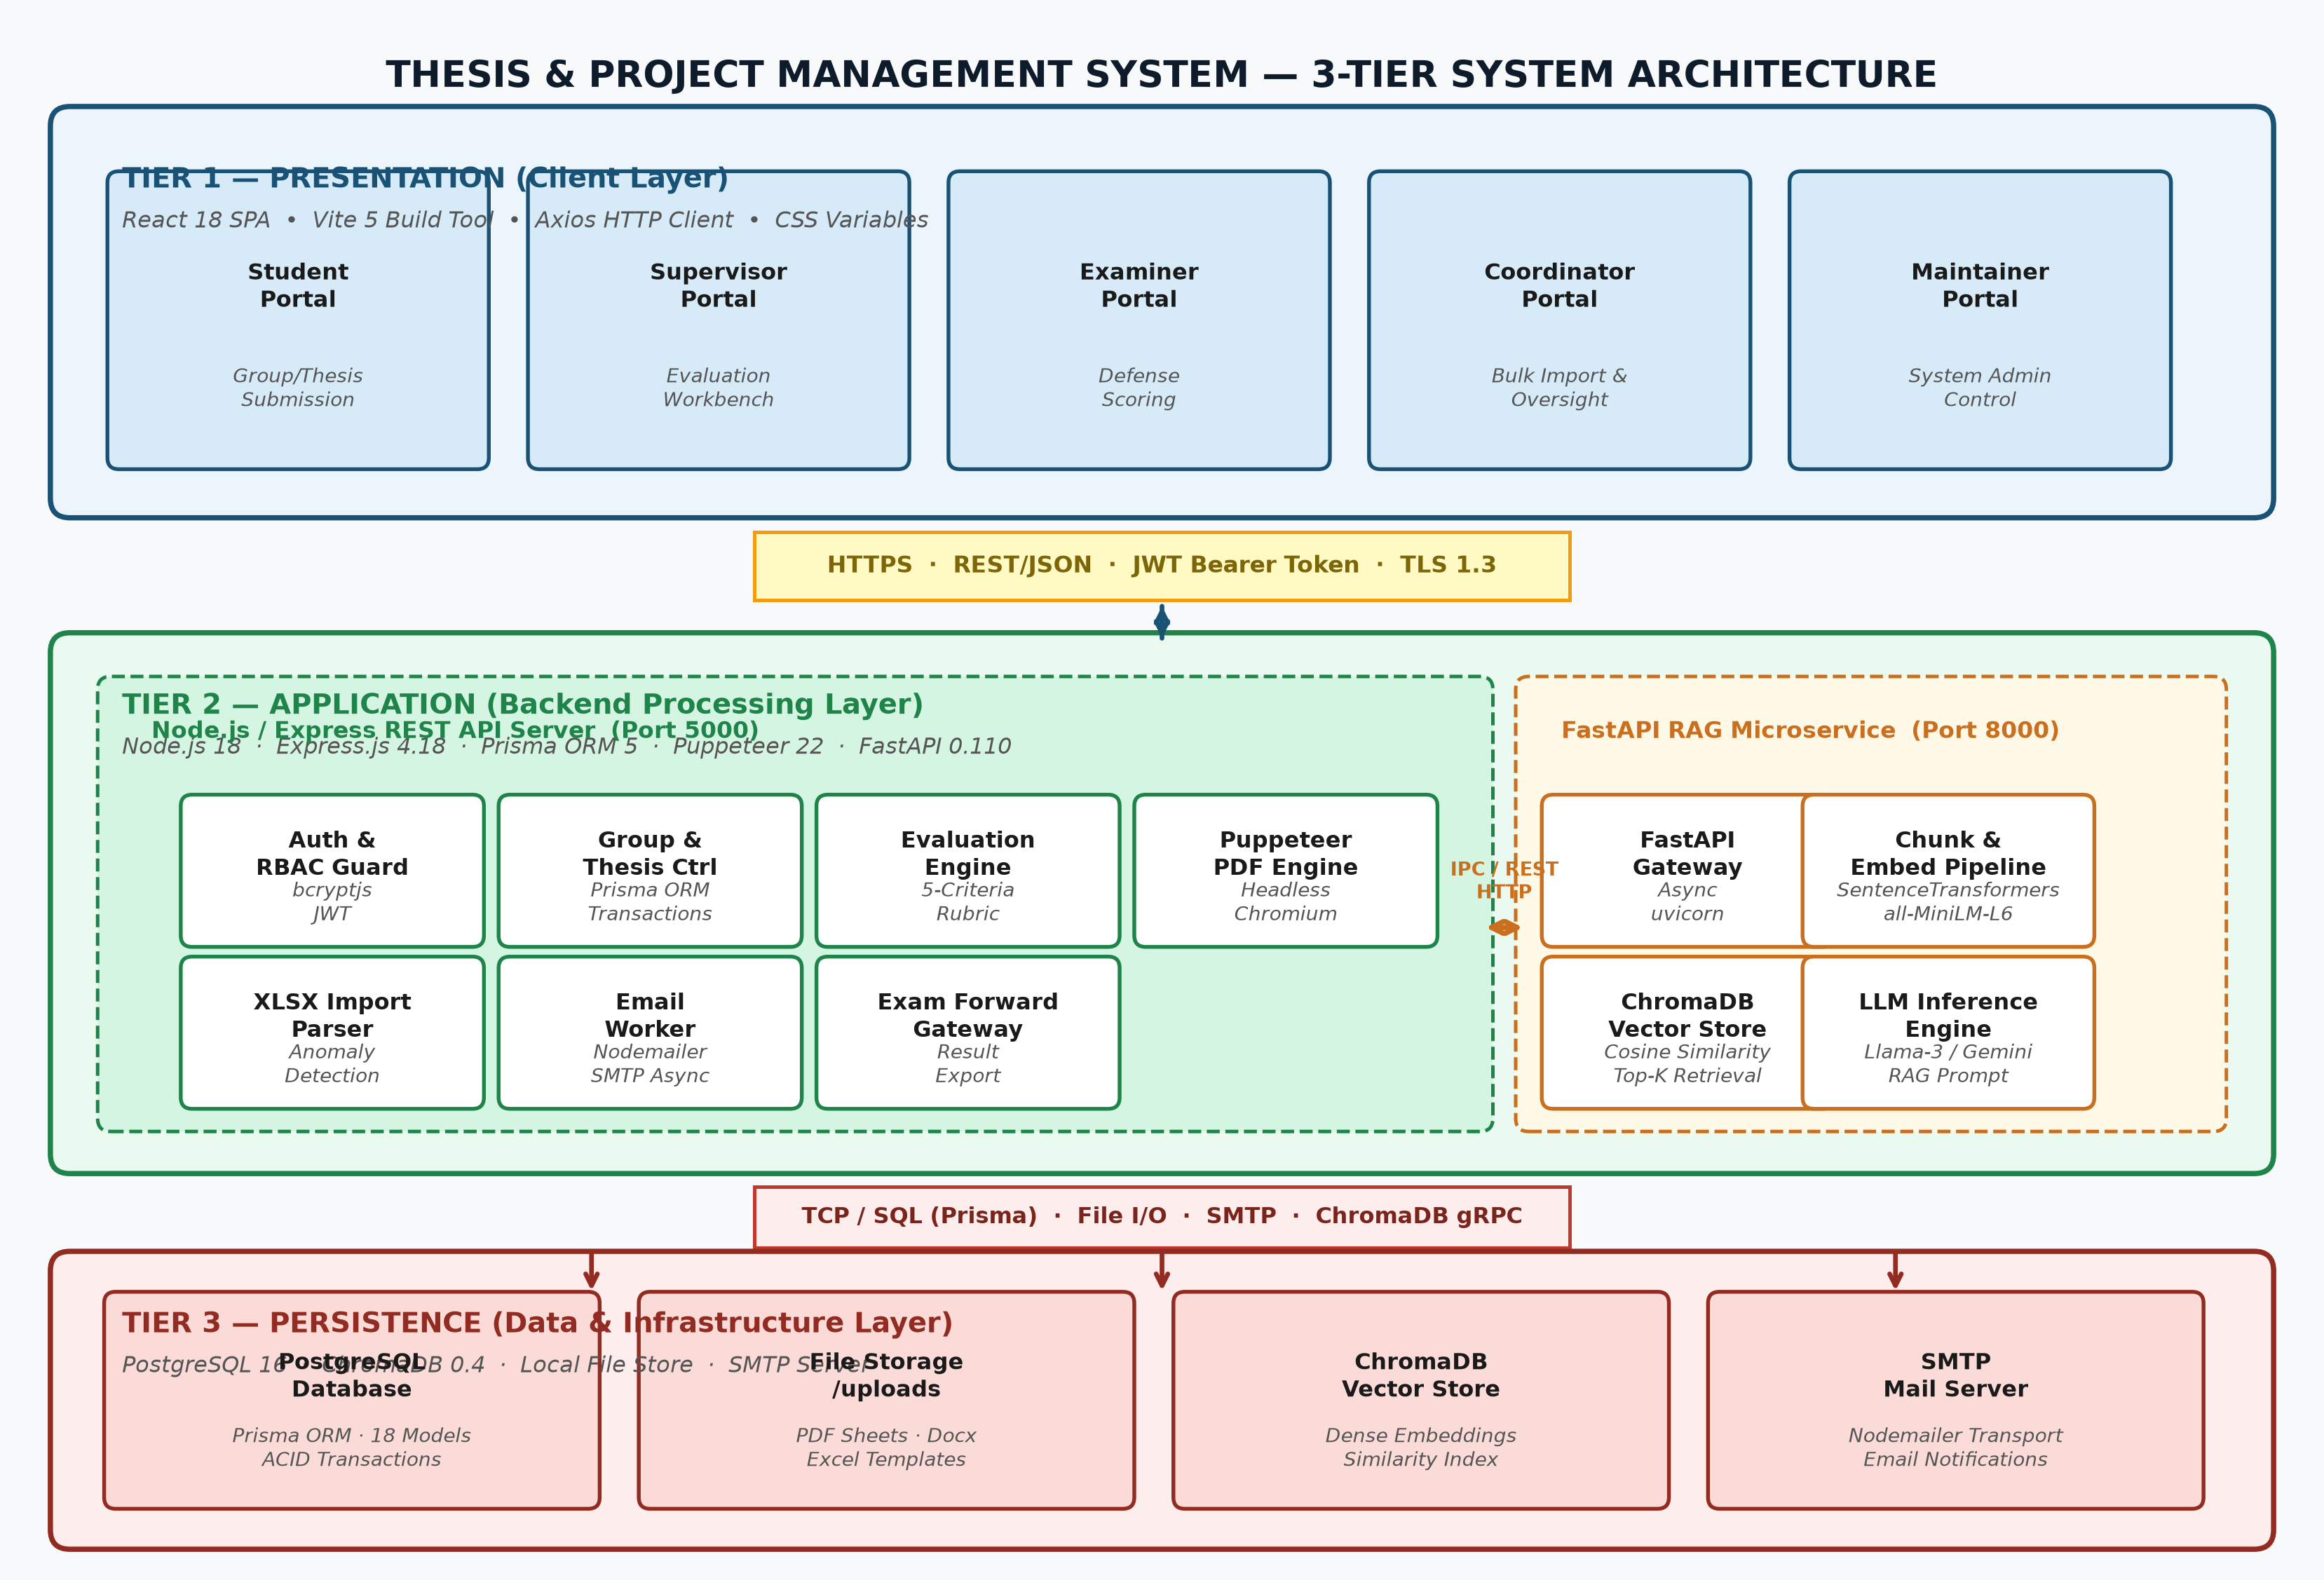
\includegraphics[width=0.98\textwidth]{fig_1_system_architecture.png}
  \caption{TPMS 3-Tier System Architecture --- Presentation, Application, and Data Layers}
  \label{fig:sys_arch}
\end{figure}

\subsection{Presentation Tier (Client Layer)}

The presentation tier is implemented as a React~18 Single-Page Application (SPA) compiled by Vite~5. All five user roles interact through a single application bundle, with React Router v6 enforcing role-based route guards. Each role receives a contextually tailored navigation menu and dashboard. Axios handles all HTTP communication with the backend API, attaching the JWT Bearer token from browser \texttt{localStorage} to every outbound request header. UI state management for cross-component data (authentication context, active program/batch selection) is handled via React Context API.

\subsection{Application Tier (Backend Processing Layer)}

The application tier comprises two independently deployed services:

\textbf{Node.js / Express REST API Server (Port 5000):} This is the primary backend processing service. It hosts all core business logic including authentication, group and thesis management, supervisor assignment, evaluation processing, and the Puppeteer PDF rendering engine. The Express server handles concurrent requests via Node.js's non-blocking event loop, making it well-suited for I/O-intensive operations such as PDF generation and SMTP dispatch.

\textbf{FastAPI RAG Microservice (Port 8000):} This Python-based microservice hosts the AI chatbot pipeline. It receives document embedding requests (proposal PDF ingestion) and natural language query requests from the main backend. The service employs SentenceTransformers for dense embedding generation and ChromaDB for vector storage and retrieval, passing retrieved context to an LLM (Llama-3 or Gemini) for answer generation.

The two backend services communicate via internal HTTP REST calls, isolating AI compute from the main application server.

\subsection{Data Tier (Persistence Layer)}

The data tier consists of four independent storage systems:

\begin{itemize}[leftmargin=*]
  \item \textbf{PostgreSQL~16:} Primary relational database housing 18 entity tables managed via Prisma ORM. Handles all transactional data: users, groups, projects, evaluations, and marks.
  \item \textbf{Local File Store (/uploads):} Server filesystem directory storing uploaded proposal PDFs, generated evaluation PDFs, and imported Excel files. Paths are stored as URL references in the database.
  \item \textbf{ChromaDB Vector Store:} Persistent vector database storing dense embeddings of ingested DOECE guideline documents and submitted proposals, enabling fast $k$-nearest-neighbor semantic search.
  \item \textbf{SMTP Mail Gateway:} Nodemailer transport configured to an SMTP server for asynchronous email notification delivery to supervisors and students.
\end{itemize}

\subsection{Inter-Tier Communication}

Communication between the presentation and application tiers uses HTTPS over TLS 1.3 with REST/JSON message format and JWT Bearer token authentication. Communication between the application tier and data tier uses PostgreSQL's native TCP wire protocol (via Prisma), filesystem I/O for file storage, gRPC for ChromaDB, and SMTP for mail dispatch.

\section{Use Case Diagram}

Figure~\ref{fig:use_case} presents the use case diagram illustrating the interactions between the five principal system actors and the eight core use case clusters.

\begin{figure}[H]
  \centering
  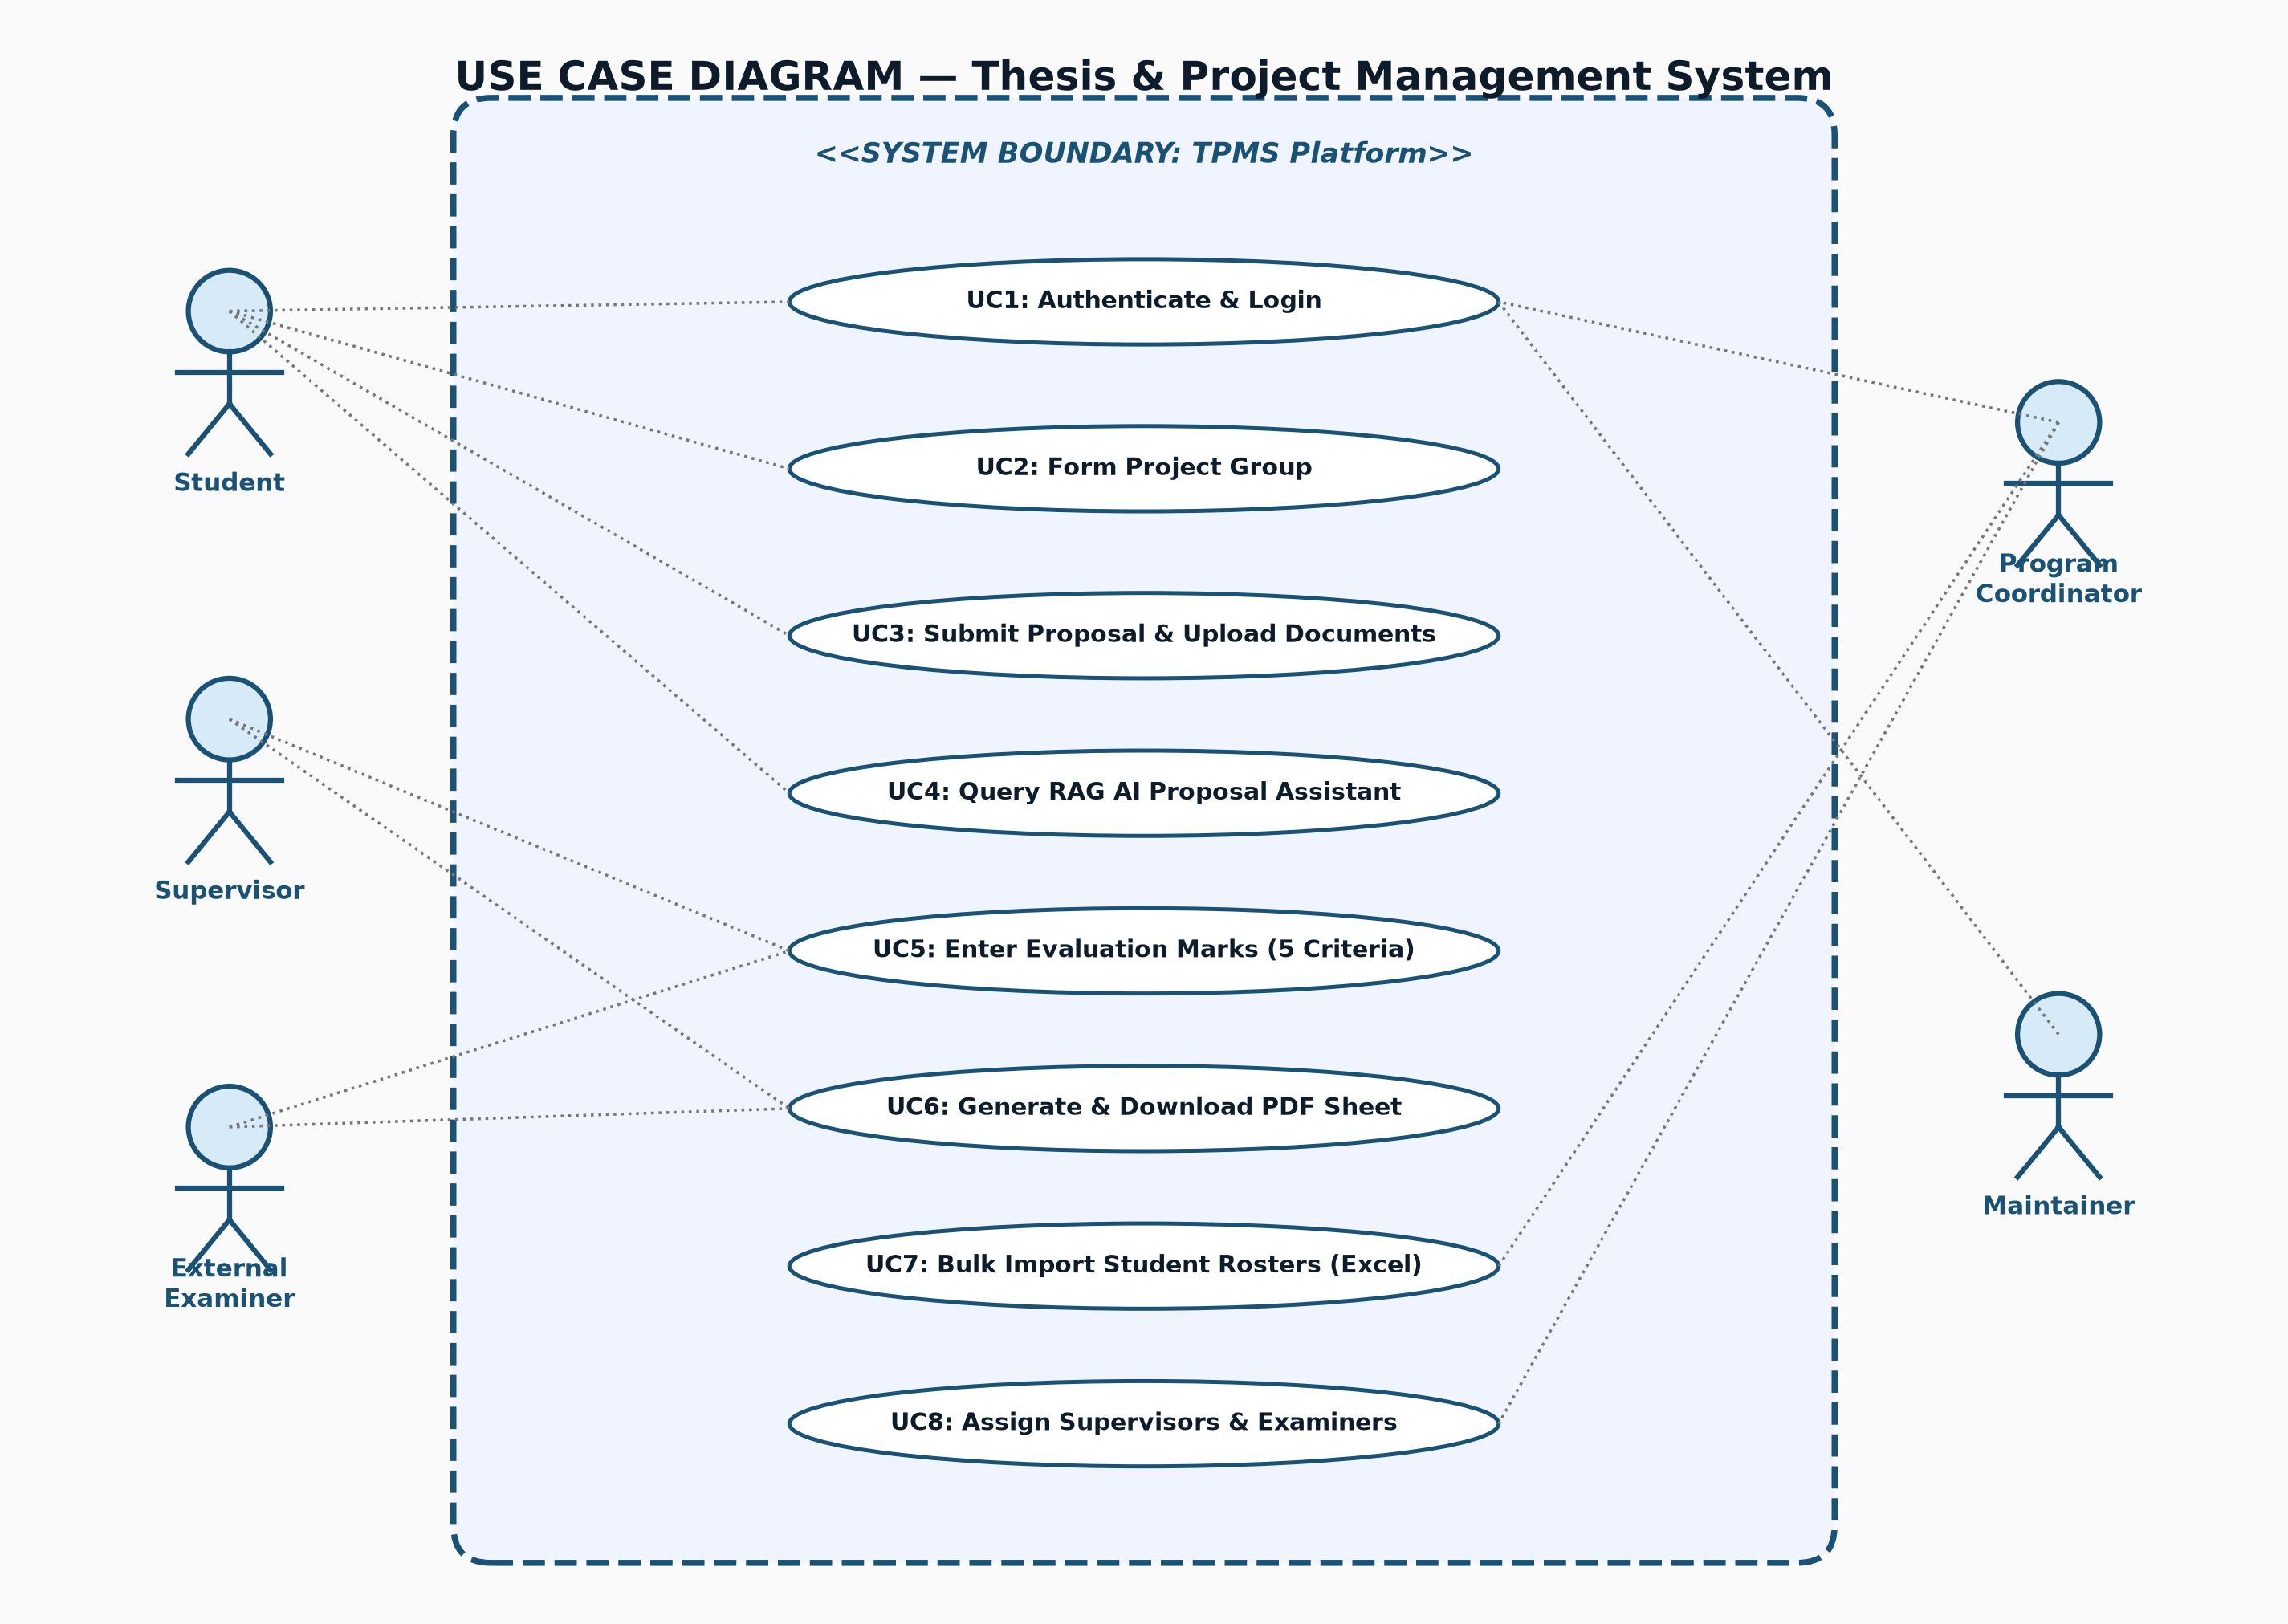
\includegraphics[width=0.92\textwidth]{fig_2_use_case_diagram.png}
  \caption{TPMS Use Case Diagram --- Actor-System Interactions}
  \label{fig:use_case}
\end{figure}

\section{Entity-Relationship Diagram}

The relational database schema of TPMS is modeled across 18 entities, of which the nine core entities and their inter-relationships are illustrated in Figure~\ref{fig:er_diagram}. All primary keys use UUID v4 for global uniqueness and distributed deployment compatibility. Foreign key constraints are enforced at the database level via Prisma migrations.

\begin{figure}[H]
  \centering
  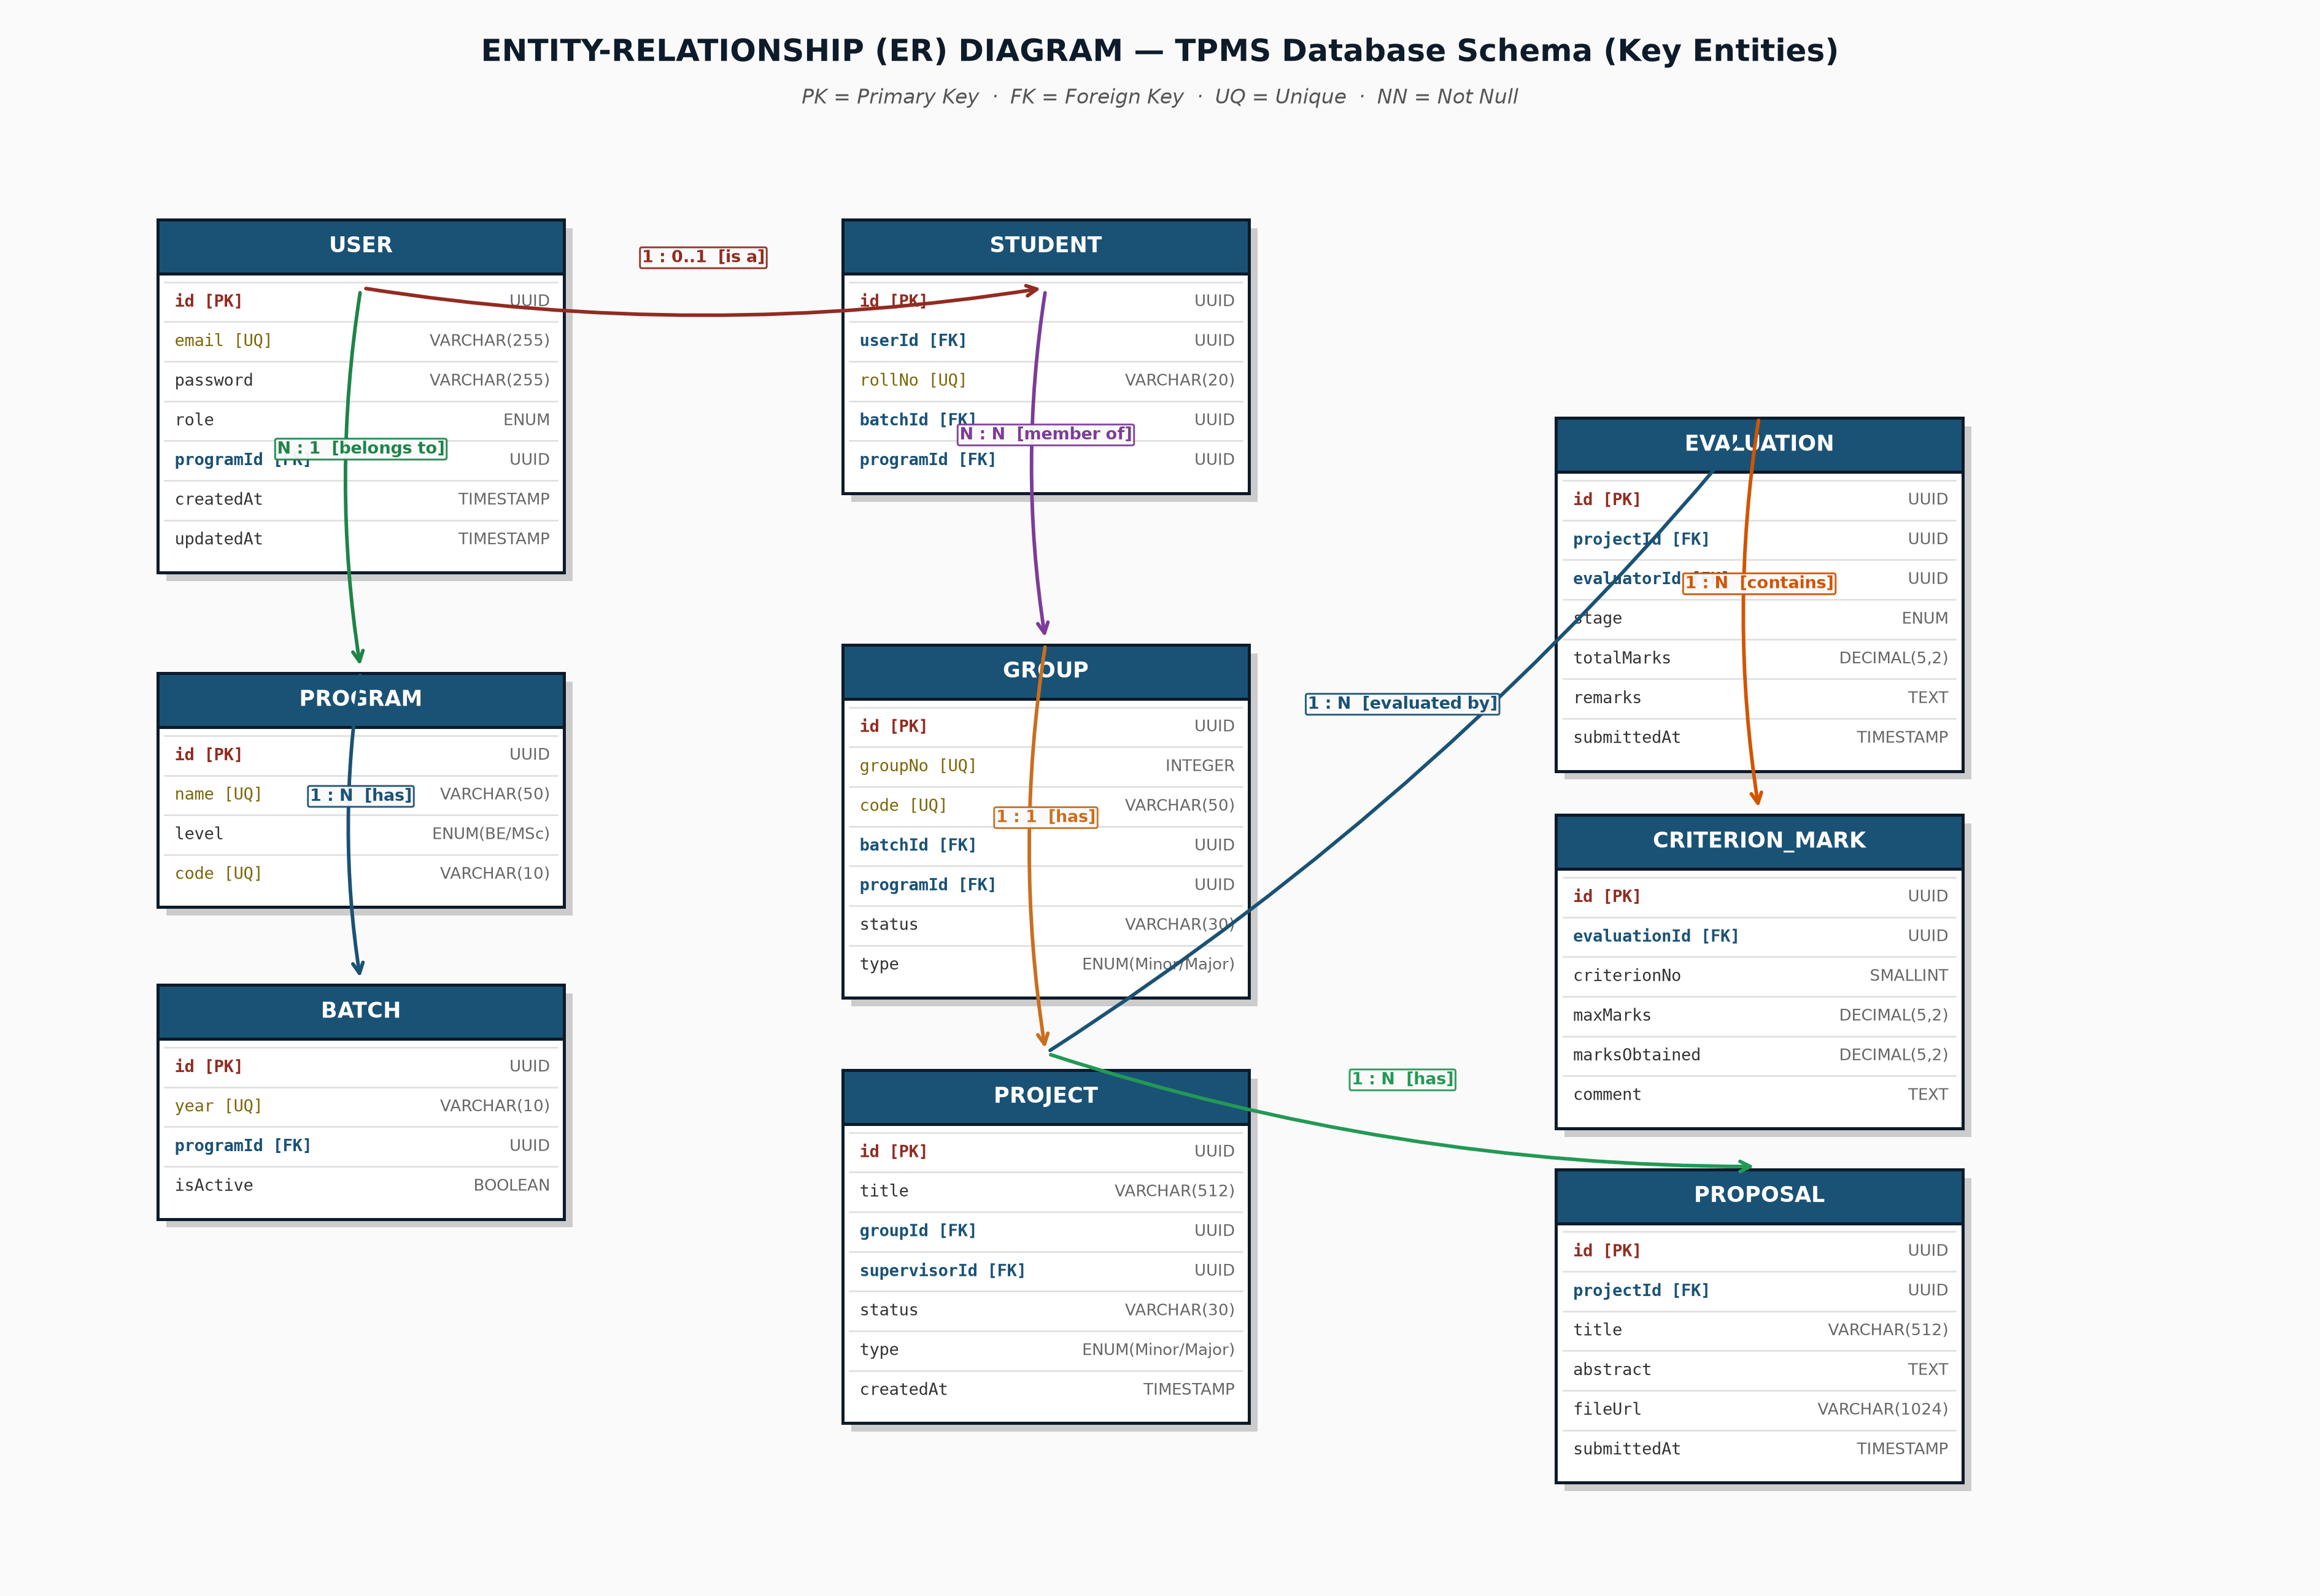
\includegraphics[width=0.98\textwidth]{fig_3_er_diagram.png}
  \caption{Entity-Relationship Diagram --- TPMS Core Database Schema with Data Types}
  \label{fig:er_diagram}
\end{figure}

Key relationships include:

\begin{itemize}[leftmargin=*]
  \item A \texttt{User} (1) maps to either a \texttt{Student} or \texttt{Faculty} record (1:0..1), capturing polymorphic role-specific profile data.
  \item A \texttt{Group} has a many-to-many relationship with \texttt{Student} (via a join table), with one active \texttt{Project} per group.
  \item A \texttt{Project} has one-to-many relationships with \texttt{Evaluation} (supervisor, mid-term, final) and \texttt{Proposal} (versioned submissions).
  \item Each \texttt{Evaluation} contains exactly five \texttt{CriterionMark} records corresponding to the five IOE evaluation criteria.
\end{itemize}

\section{Data Flow Diagram (Level 1)}

Figure~\ref{fig:dfd1} presents the Level~1 Data Flow Diagram for TPMS using Yourdon-Coad notation. External entities (students, supervisors, examiners, and coordinator) interact with six processing nodes through six data stores.

\begin{figure}[H]
  \centering
  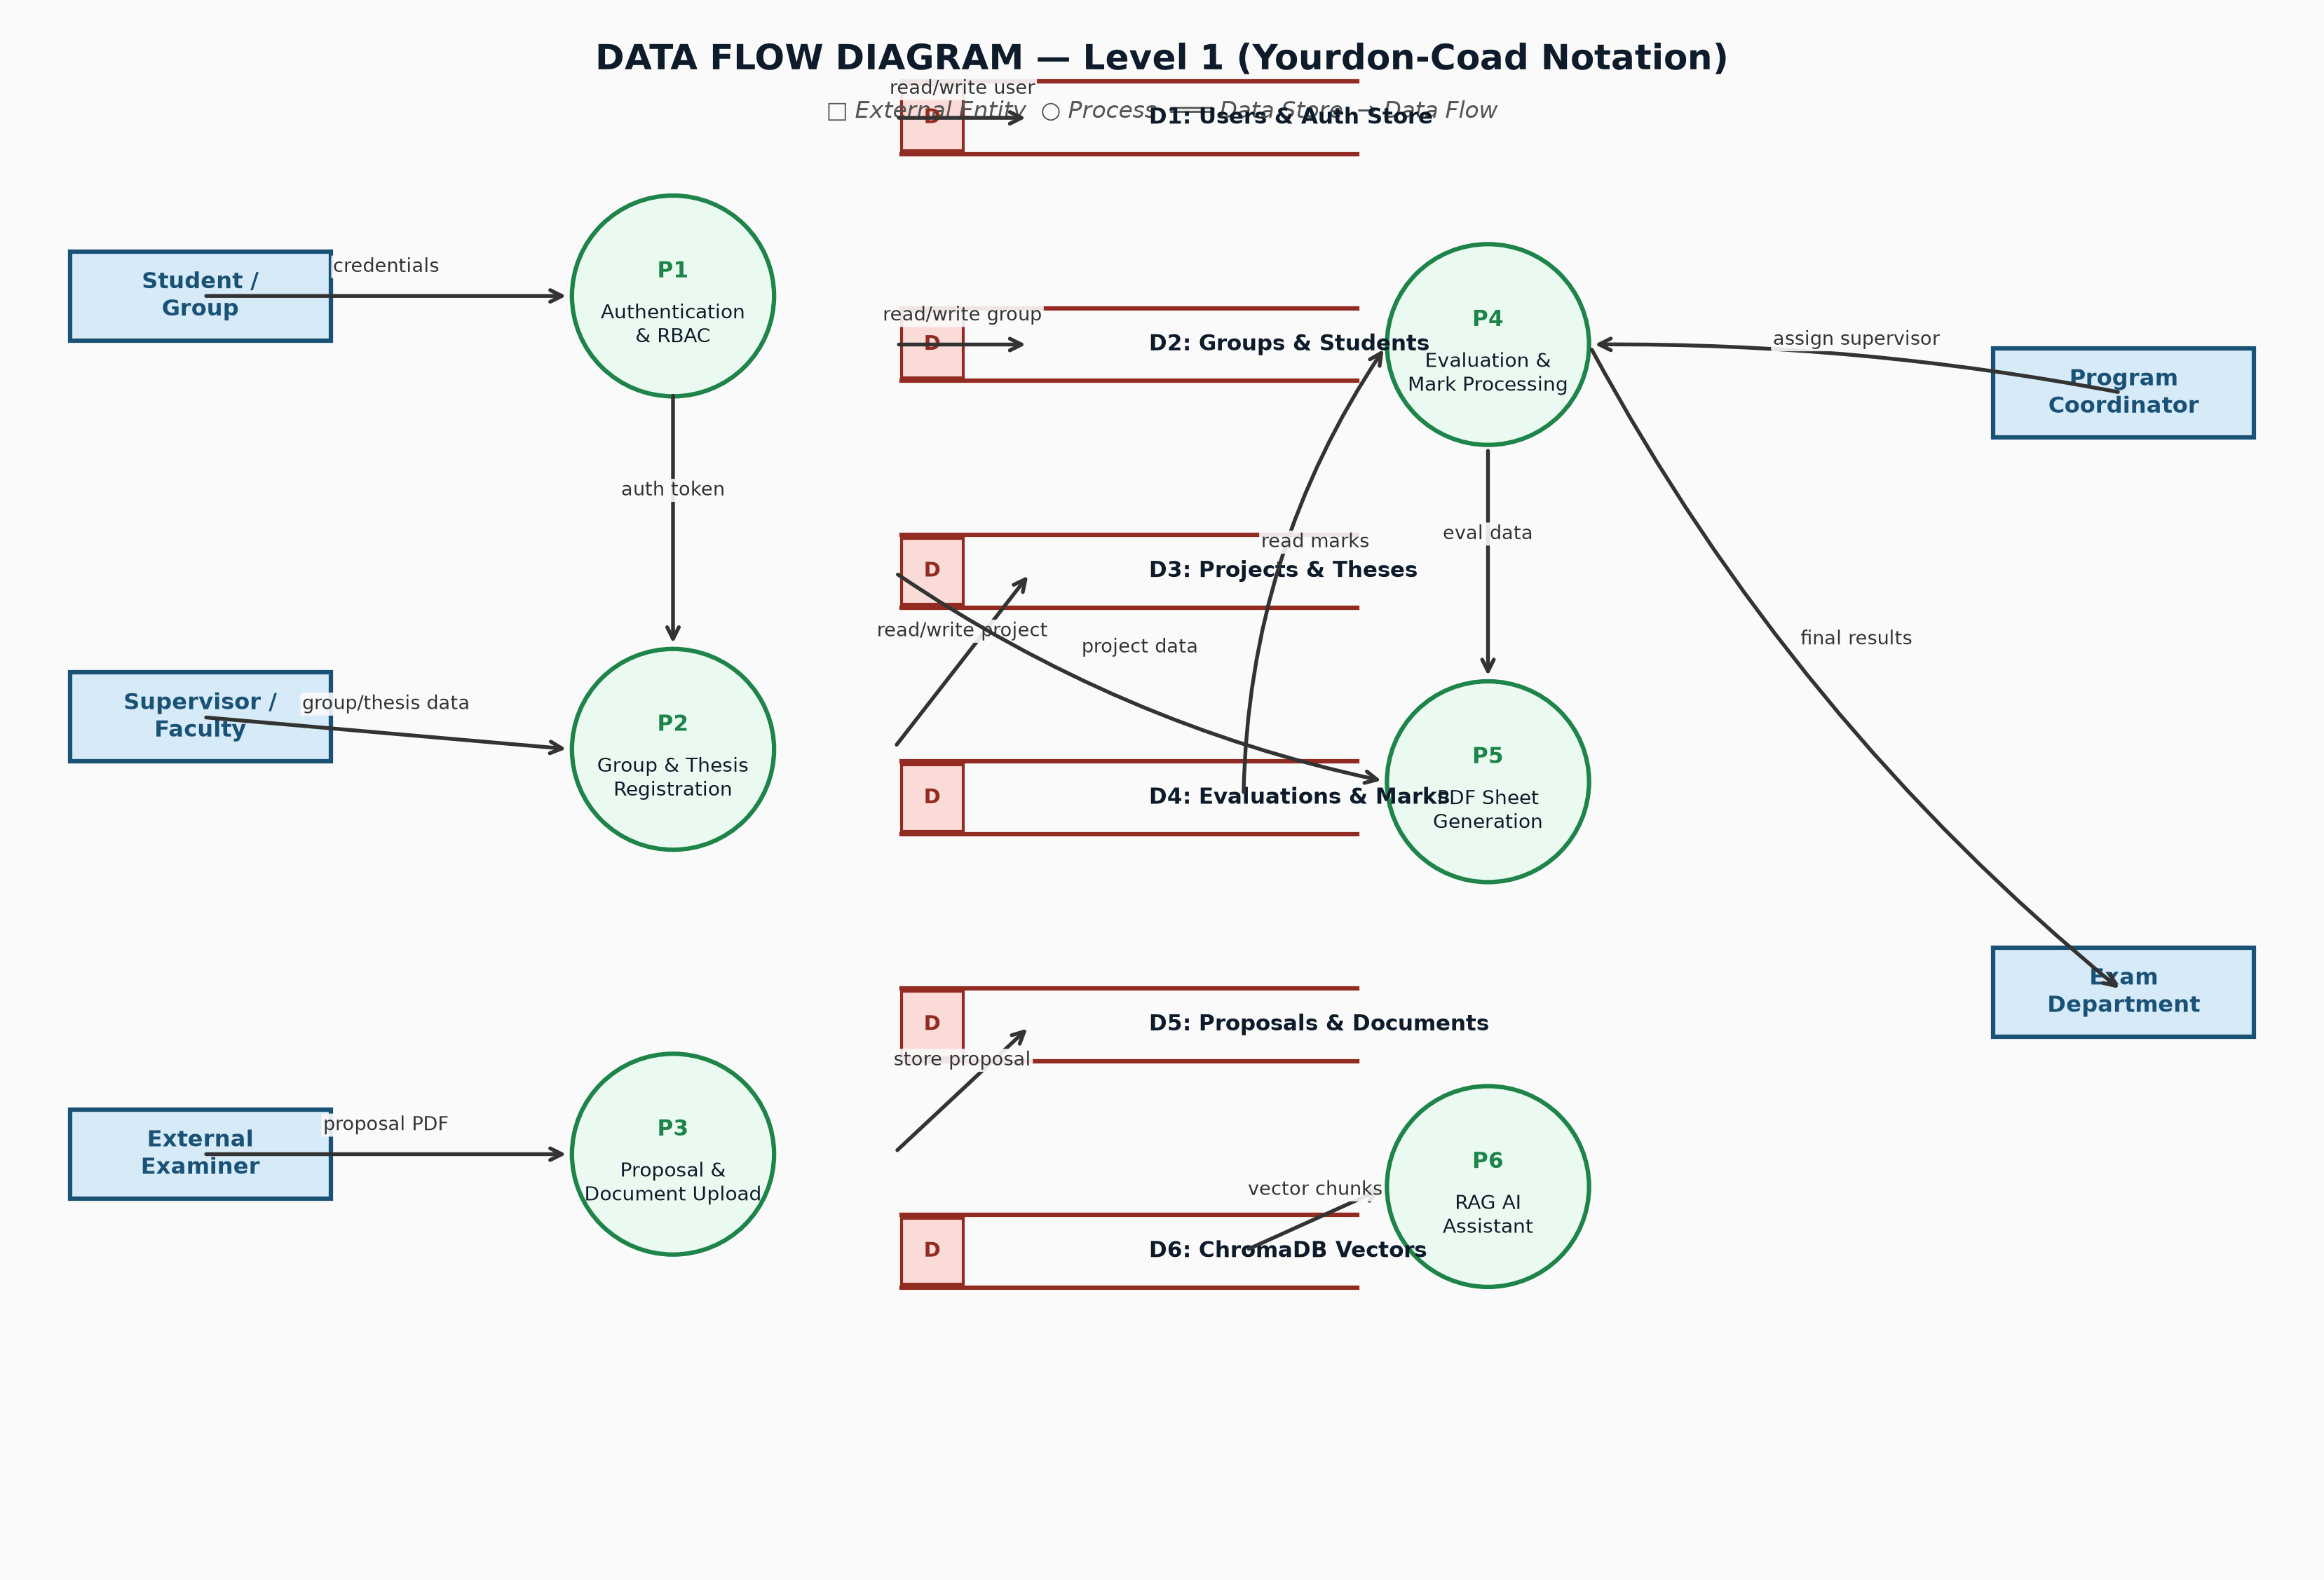
\includegraphics[width=0.98\textwidth]{fig_7_dfd_level_1.png}
  \caption{Data Flow Diagram (Level 1, Yourdon-Coad Notation)}
  \label{fig:dfd1}
\end{figure}

\section{Behavioral Diagrams}

\subsection{Excel Batch Import Sequence}

The sequence diagram in Figure~\ref{fig:seq_import} illustrates the two-phase Excel bulk import workflow. Phase~1 (preview) parses the uploaded file and returns anomaly reports without committing any database changes. Phase~2 (confirm) executes the full transactional creation of groups, students, and supervisor assignments.

\begin{figure}[H]
  \centering
  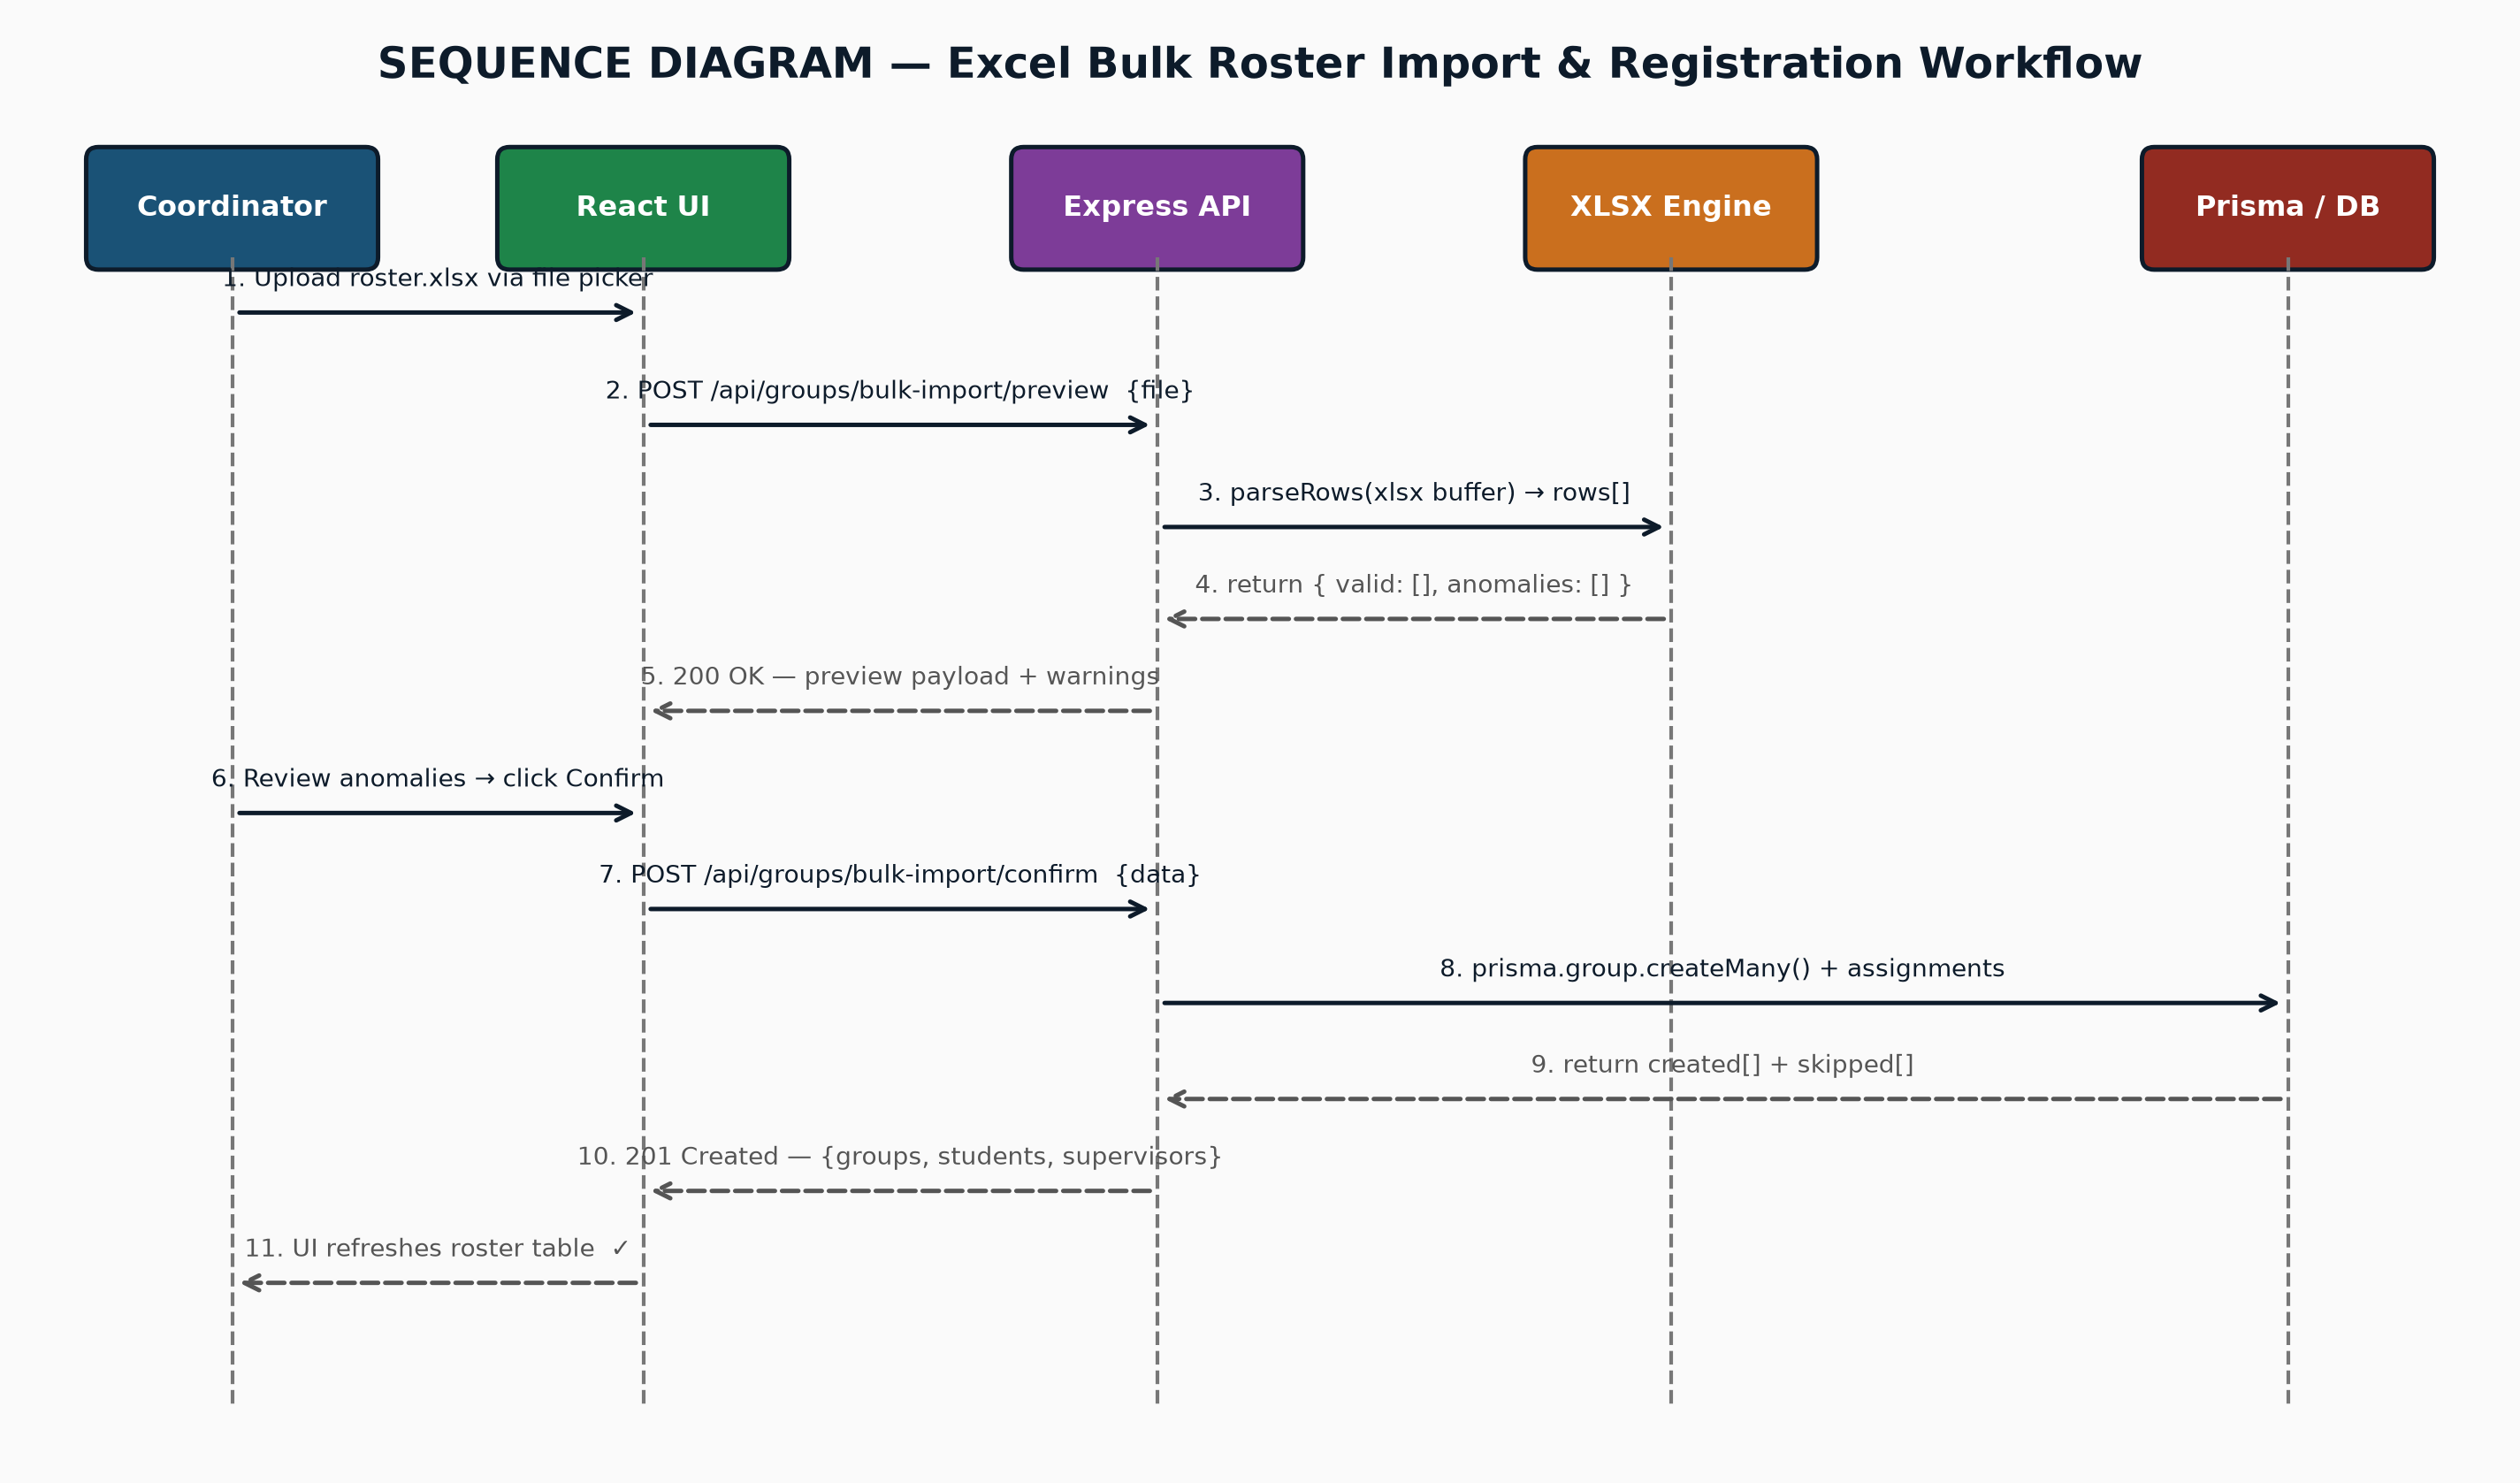
\includegraphics[width=0.95\textwidth]{fig_4_excel_import_sequence.png}
  \caption{Sequence Diagram: Excel Bulk Roster Import \& Registration Workflow}
  \label{fig:seq_import}
\end{figure}

\subsection{Supervisor Assignment Sequence}

Figure~\ref{fig:seq_assign} illustrates the supervisor assignment flow, including the non-blocking email dispatch pattern. The API returns the HTTP~200 confirmation immediately after the database commit, while the Nodemailer SMTP worker delivers the notification email asynchronously in a background queue, avoiding API latency degradation.

\begin{figure}[H]
  \centering
  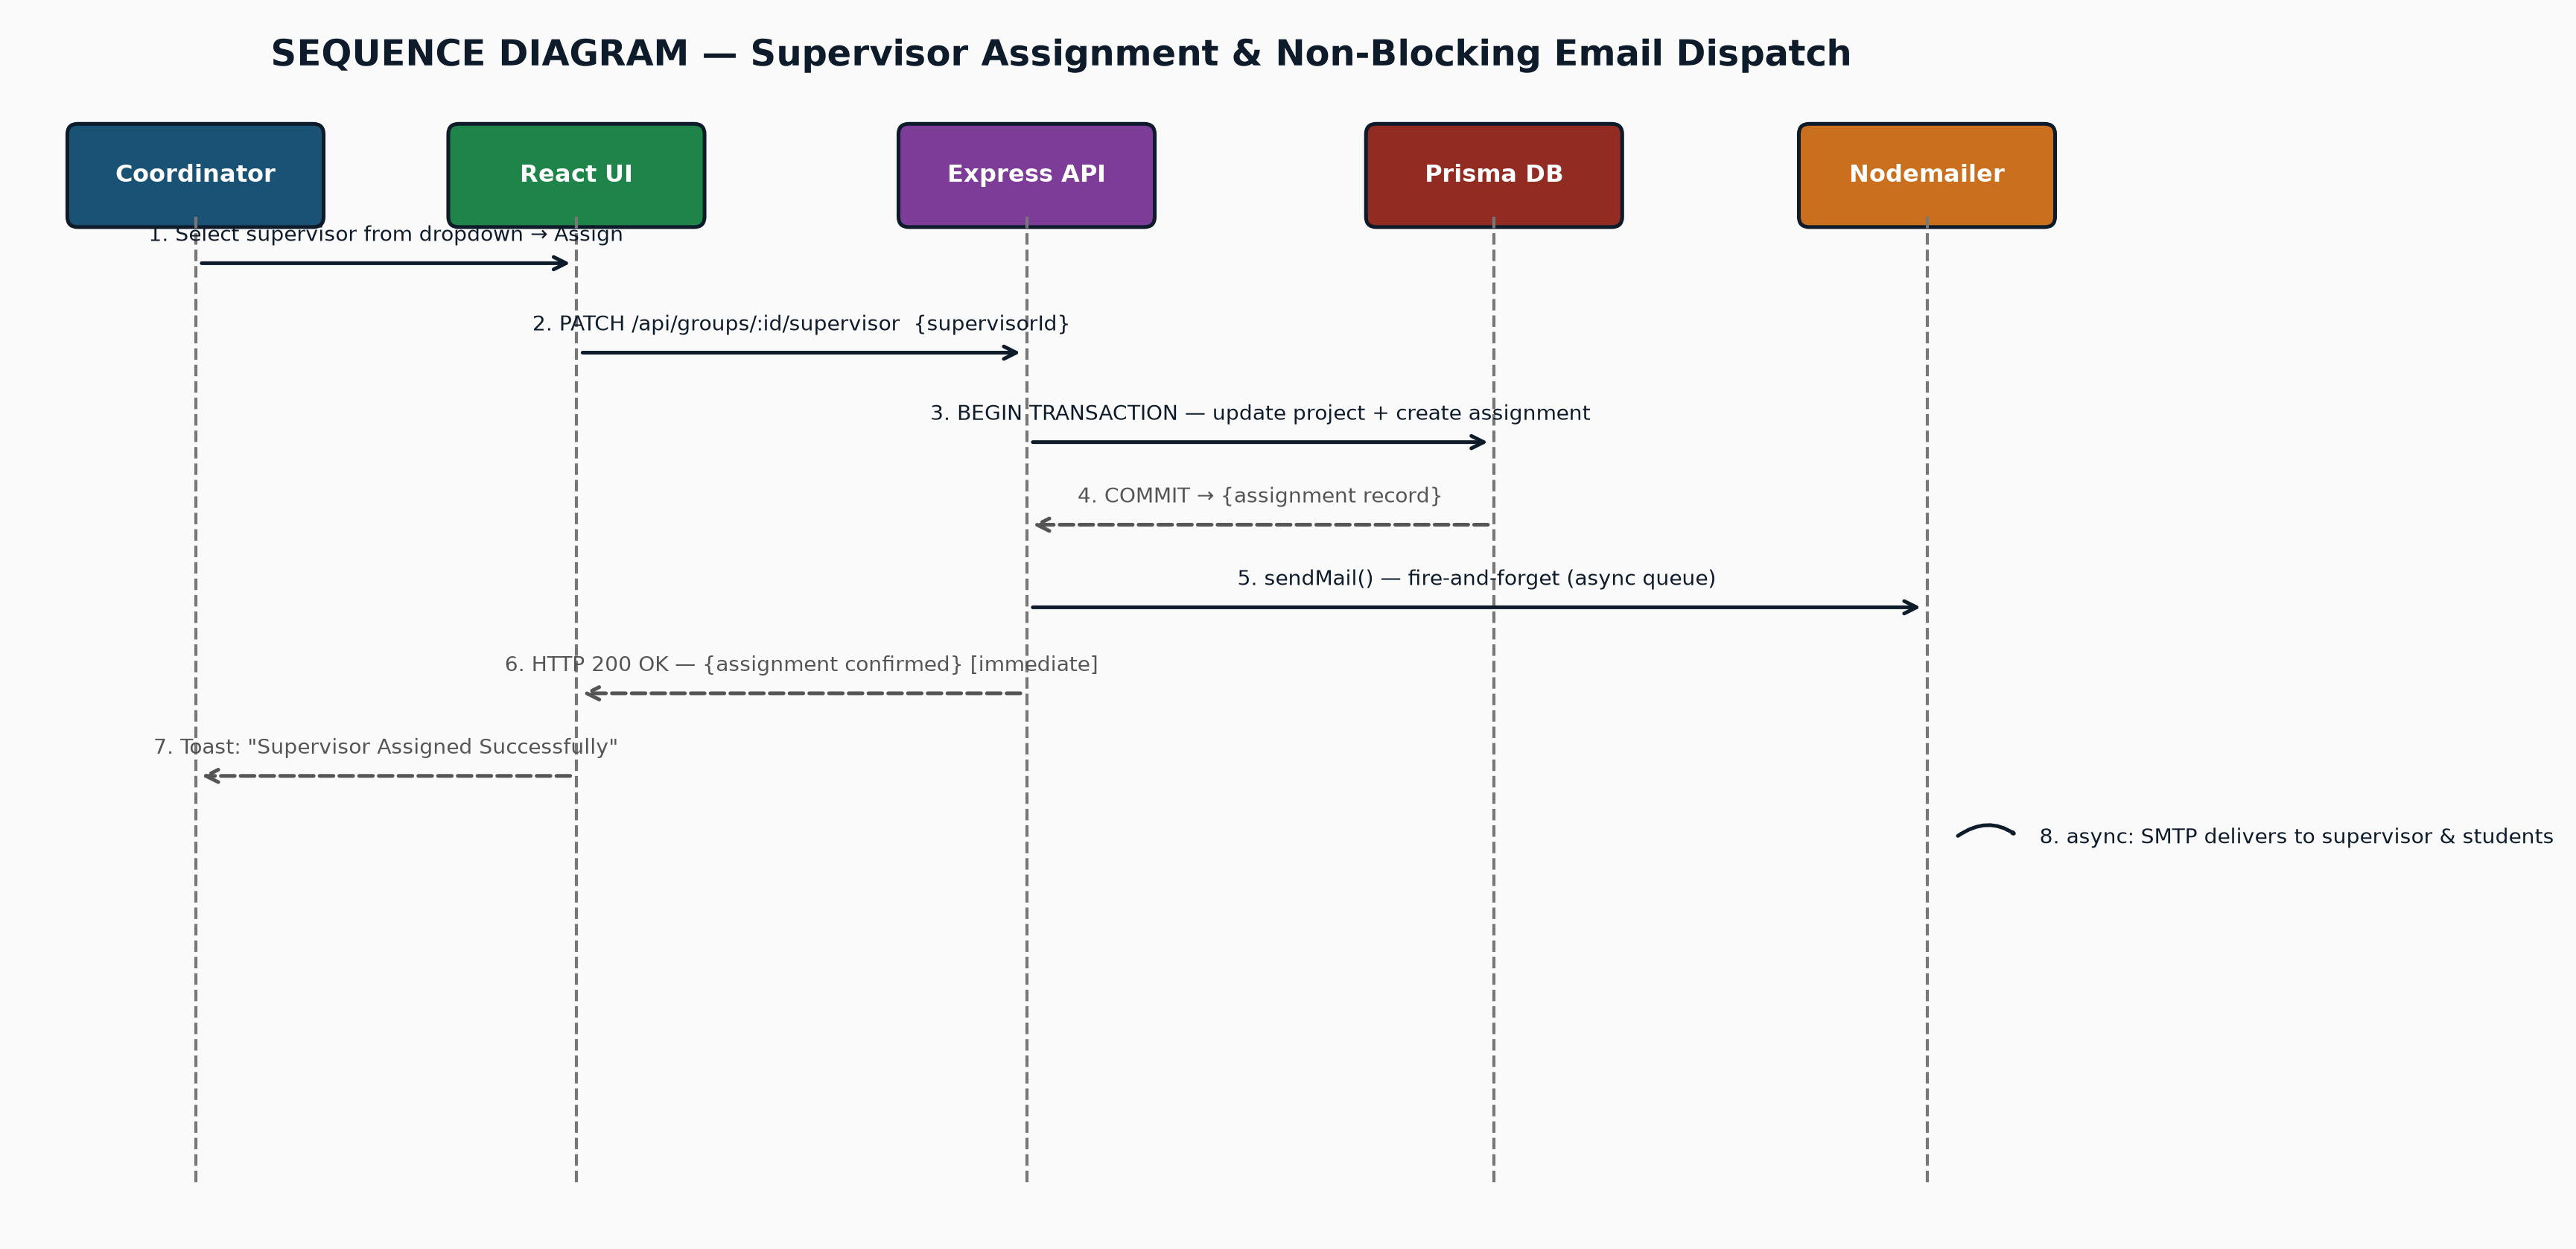
\includegraphics[width=0.95\textwidth]{fig_5_supervisor_assignment_flow.png}
  \caption{Sequence Diagram: Supervisor Assignment \& Non-Blocking Email Dispatch}
  \label{fig:seq_assign}
\end{figure}

\subsection{Evaluation \& PDF Generation Sequence}

Figure~\ref{fig:seq_eval} details the marks submission and Puppeteer PDF generation lifecycle. The evaluation API inserts five \texttt{CriterionMark} records transactionally, computes the total, and triggers the PDF rendering engine which constructs an HTML evaluation sheet template, launches a headless Chromium instance via Puppeteer, renders the page to PDF, and streams the binary buffer back to the browser for inline preview.

\begin{figure}[H]
  \centering
  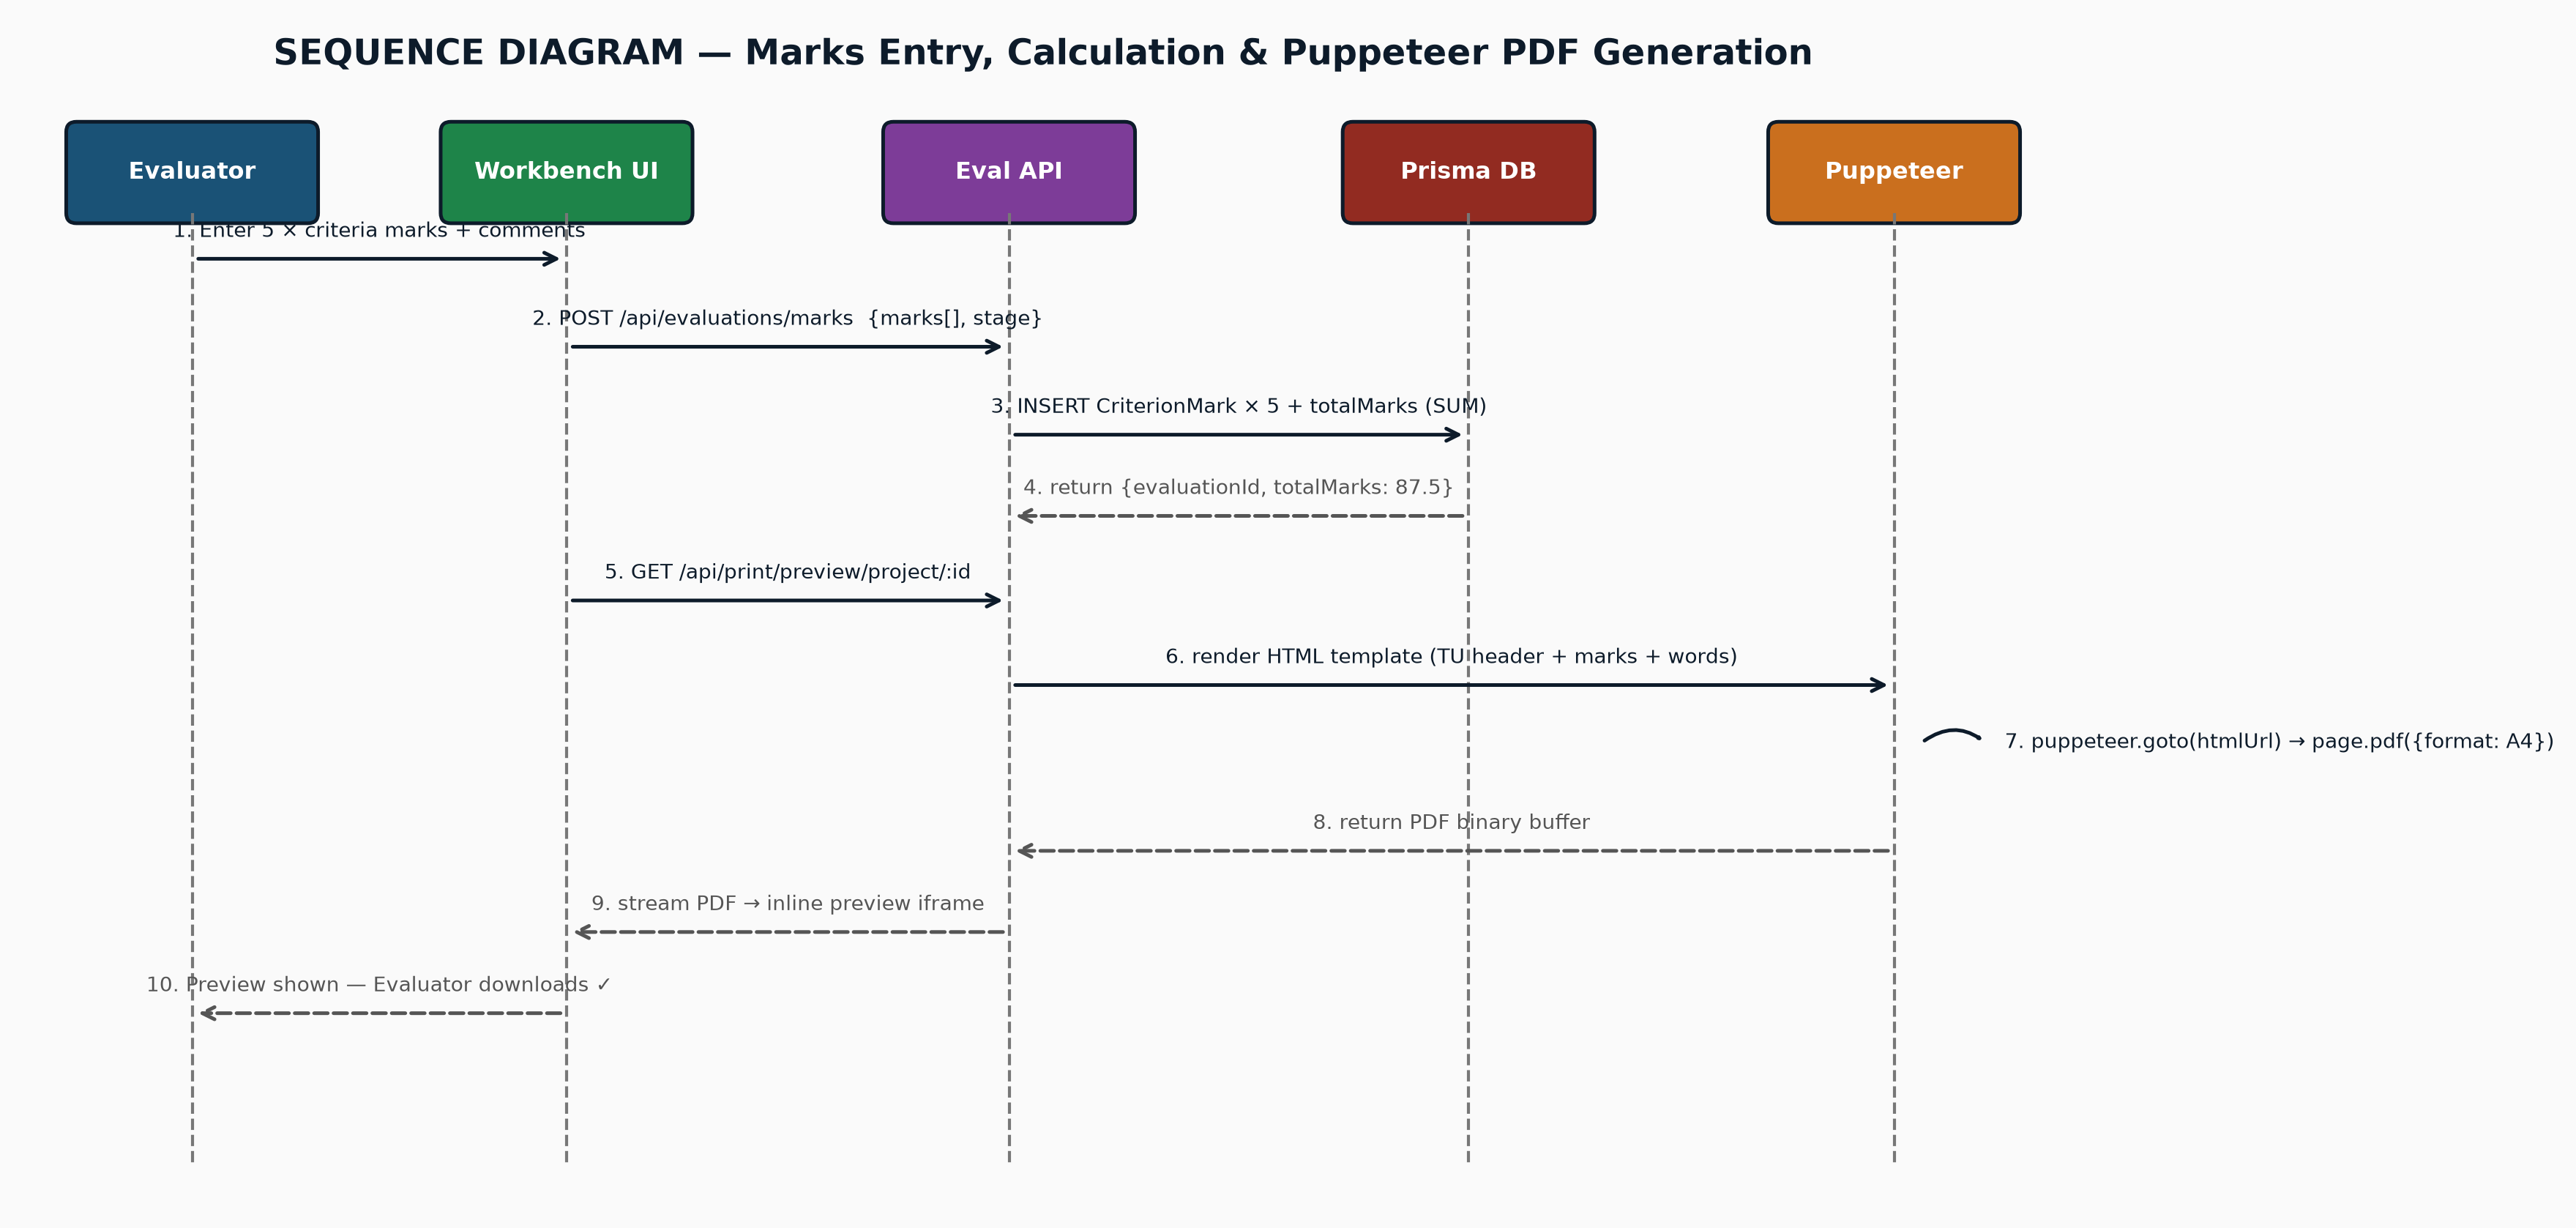
\includegraphics[width=0.95\textwidth]{fig_6_evaluation_submission_sequence.png}
  \caption{Sequence Diagram: Marks Entry, Calculation \& Puppeteer PDF Generation}
  \label{fig:seq_eval}
\end{figure}

\section{Project Schedule}

The 16-week project development timeline organized by engineering phase is presented in the Gantt chart in Figure~\ref{fig:gantt}.

\begin{figure}[H]
  \centering
  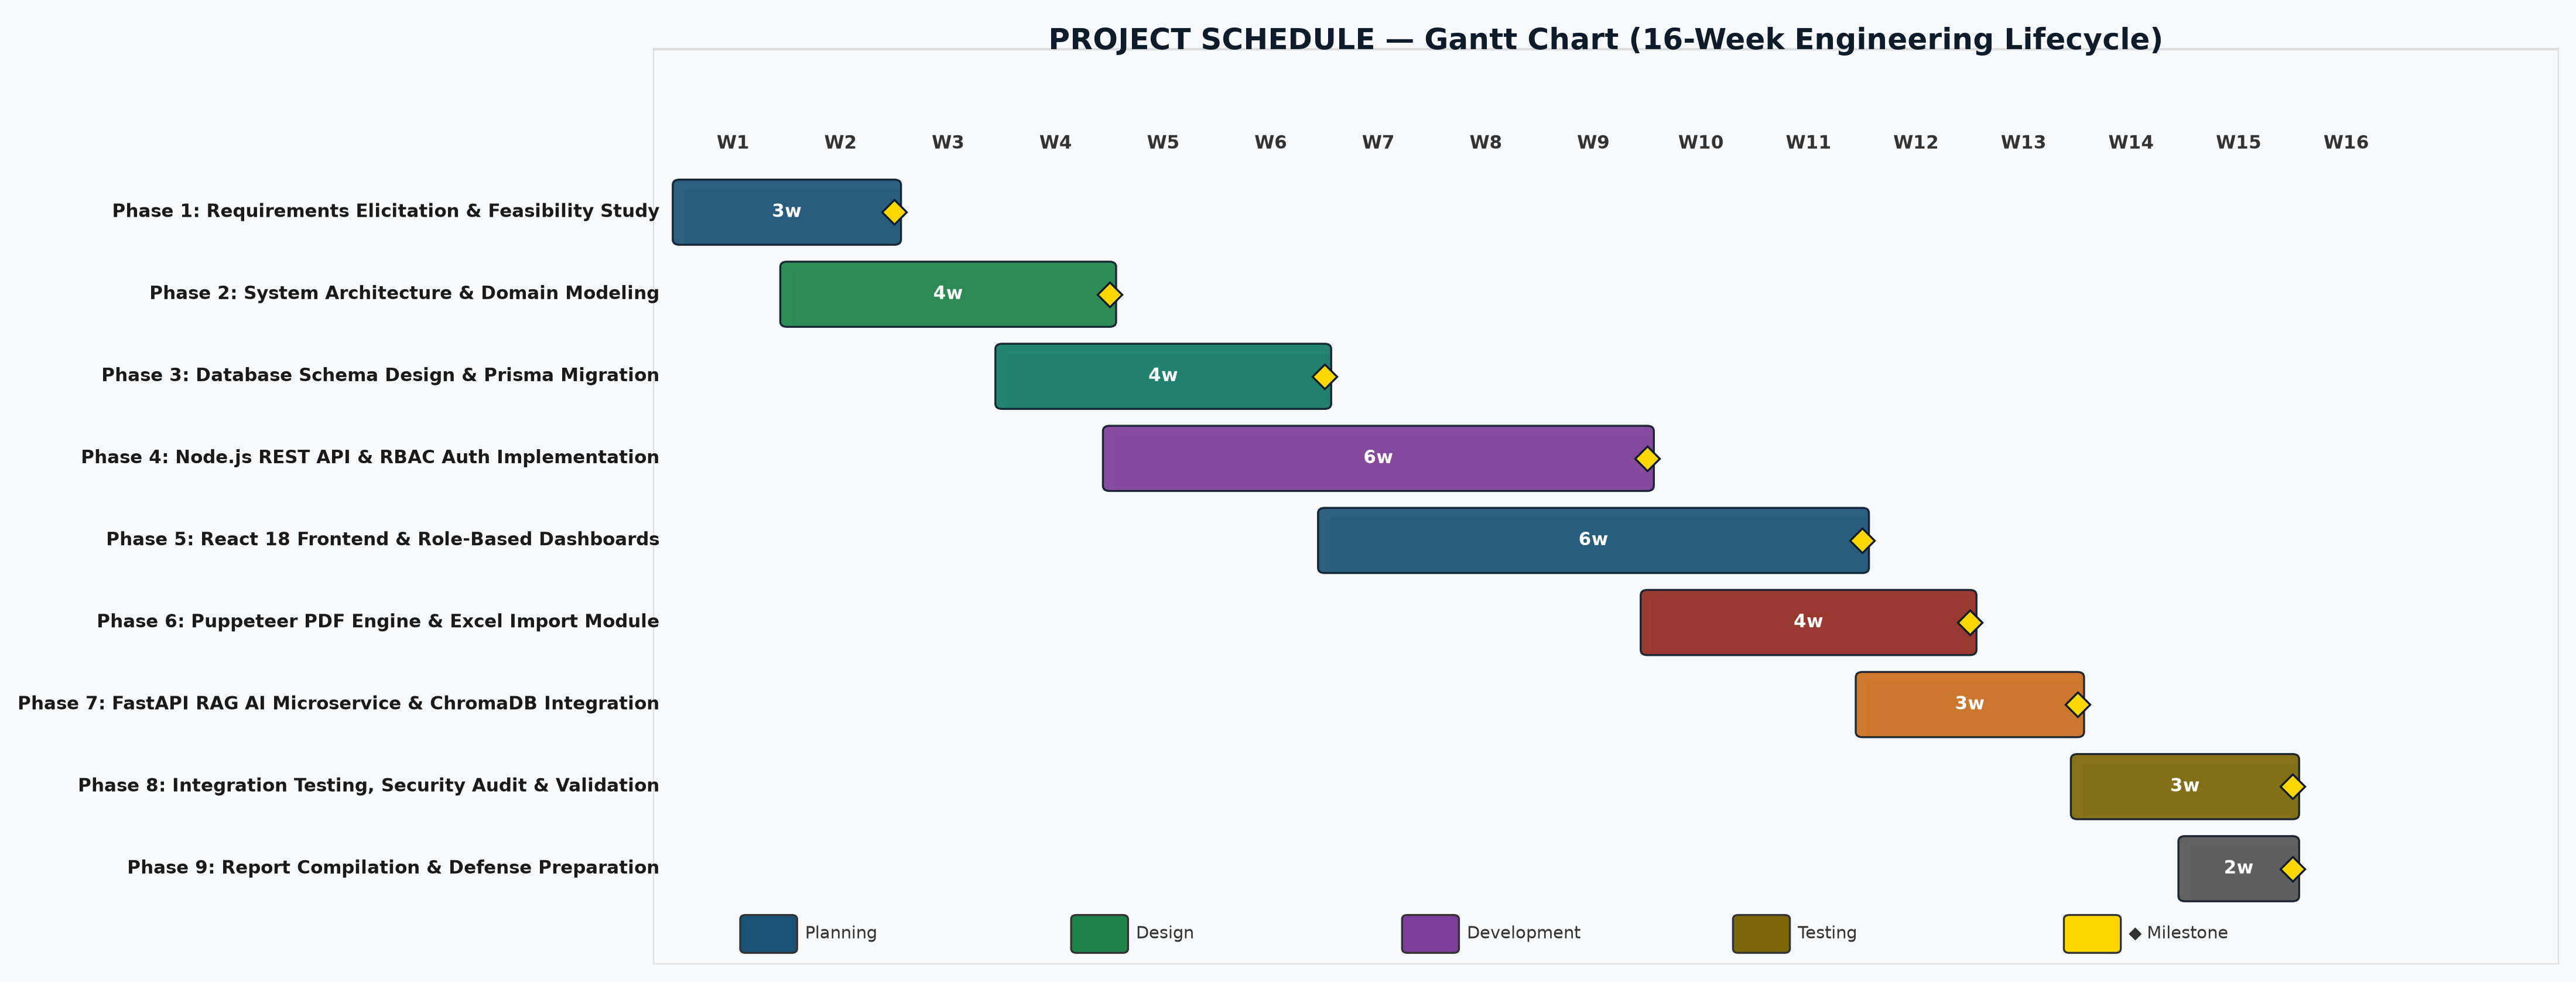
\includegraphics[width=0.98\textwidth]{fig_8_gantt_chart.png}
  \caption{Project Development Gantt Chart (16-Week Engineering Lifecycle)}
  \label{fig:gantt}
\end{figure}

%% ══════════════════════════════════════════════════════════════════════════════
\chapter{Experimental Setup \& Implementation}
%% ══════════════════════════════════════════════════════════════════════════════

\section{Development Environment}

The system was implemented and tested on a Linux development environment. Table~\ref{tab:env_config} summarizes the complete hardware and software configuration.

\begin{table}[H]
\centering
\caption{System Environment Configuration}\label{tab:env_config}
\begin{tabular}{l l}
\toprule
\textbf{Component} & \textbf{Specification / Version}\\
\midrule
Operating System & Ubuntu 22.04 LTS / Fedora 40 (development)\\
Runtime (Backend) & Node.js v18.19.0 (LTS)\\
Runtime (AI Service) & Python 3.11.5\\
Database & PostgreSQL 16.2 with pgAdmin 4\\
ORM & Prisma 5.10.0\\
Frontend Framework & React 18.2.0 + Vite 5.1.0\\
PDF Engine & Puppeteer 22.3.0 (Headless Chromium 123)\\
AI Framework & FastAPI 0.110.0 + ChromaDB 0.4.24\\
LLM & Llama-3-8B-Instruct / Gemini 1.5 Flash\\
HTTP Server & Express.js 4.18.2\\
Auth Library & jsonwebtoken 9.0.0 + bcryptjs 2.4.3\\
Email & Nodemailer 6.9.7\\
Excel Parser & xlsx (SheetJS) 0.18.5\\
Testing & Jest 29.7.0 + Supertest 6.3.4\\
Version Control & Git 2.43.0 + GitHub\\
\bottomrule
\end{tabular}
\end{table}

\section{Database Schema Implementation}

The Prisma schema defines 18 models with complete type safety. The core models are defined using UUID primary keys, enum-typed role and status fields, and explicit foreign key references for relational integrity. A representative schema excerpt is shown below:

\begin{lstlisting}[language=Java, caption={Prisma Schema --- Group \& Evaluation Models}]
model Group {
  id             String       @id @default(uuid())
  groupNo        Int
  code           String       @unique
  type           ProjectType  // Minor | Major
  status         GroupStatus
  batchId        String
  programId      String
  batch          Batch        @relation(fields: [batchId], references: [id])
  program        Program      @relation(fields: [programId], references: [id])
  members        StudentGroup[]
  project        Project?
  createdAt      DateTime     @default(now())
}

model Evaluation {
  id             String          @id @default(uuid())
  projectId      String
  evaluatorId    String
  stage          EvaluationStage  // SUPERVISOR | MID_TERM | FINAL
  totalMarks     Decimal         @db.Decimal(5, 2)
  remarks        String?
  marks          CriterionMark[]
  submittedAt    DateTime        @default(now())
  project        Project         @relation(fields: [projectId], references: [id])
}

model CriterionMark {
  id             String     @id @default(uuid())
  evaluationId   String
  criterionNo    Int        @db.SmallInt
  maxMarks       Decimal    @db.Decimal(5, 2)
  marksObtained  Decimal    @db.Decimal(5, 2)
  comment        String?
  evaluation     Evaluation @relation(fields: [evaluationId], references: [id])
}
\end{lstlisting}

\section{PDF Rendering Engine Implementation}

The Puppeteer PDF engine generates official IOE evaluation sheets by dynamically injecting evaluation data into an HTML template with precise CSS Paged Media formatting. A critical utility converts numerical totals to English word equivalents as required by IOE format:

\begin{lstlisting}[language=Java, caption={Numerical-to-Word Mark Conversion Utility}]
function numberToWords(num) {
  const units = ['', 'One', 'Two', 'Three', 'Four', 'Five',
                 'Six', 'Seven', 'Eight', 'Nine'];
  const teens = ['Ten', 'Eleven', 'Twelve', 'Thirteen', 'Fourteen',
                 'Fifteen', 'Sixteen', 'Seventeen', 'Eighteen', 'Nineteen'];
  const tens  = ['', '', 'Twenty', 'Thirty', 'Forty', 'Fifty',
                 'Sixty', 'Seventy', 'Eighty', 'Ninety'];
  if (num === 0) return 'Zero';
  const parts = num.toString().split('.');
  let n = parseInt(parts[0]), result = '';
  if (n >= 100) {
    result += units[Math.floor(n / 100)] + ' Hundred ';
    n %= 100;
  }
  if (n >= 10 && n <= 19) result += teens[n - 10] + ' ';
  else if (n >= 20) result += tens[Math.floor(n/10)] + ' ' + units[n%10] + ' ';
  else if (n > 0) result += units[n] + ' ';
  if (parts.length > 1)
    result += 'Point ' + [...parts[1]].map(c => units[+c]).join(' ');
  return result.trim() + ' Only';
}

// Puppeteer PDF compilation
const browser = await puppeteer.launch({ args: ['--no-sandbox'] });
const page    = await browser.newPage();
await page.setContent(htmlTemplate, { waitUntil: 'networkidle0' });
const pdfBuffer = await page.pdf({
  format: 'A4', margin: { top: '15mm', right: '15mm',
                           bottom: '15mm', left: '15mm' },
  printBackground: true,
});
await browser.close();
\end{lstlisting}

\section{RAG AI Microservice Setup}

The RAG pipeline is implemented in FastAPI with ChromaDB as the vector store. Submitted proposal PDFs are parsed using PyMuPDF into 1000-character text chunks with 200-character overlap. Embeddings are computed using \texttt{all-MiniLM-L6-v2} SentenceTransformer and indexed in ChromaDB. At query time, the user's question is embedded, and the top-3 most semantically similar chunks are retrieved and prepended into the LLM prompt:

\begin{lstlisting}[language=Python, caption={FastAPI RAG Query Endpoint}]
@app.post("/api/ai/query")
async def query_rag(req: QueryRequest):
    query_embedding = embedding_model.encode([req.question]).tolist()
    results = collection.query(
        query_embeddings=query_embedding,
        n_results=3
    )
    context = "\n\n".join(results['documents'][0])
    prompt = f"""You are a DOECE project guideline assistant.
    
Context from guidelines:
{context}

Student question: {req.question}

Provide a concise, accurate answer based only on the provided context."""
    response = llm_client.generate(prompt)
    return {"answer": response, "sources": results['ids'][0]}
\end{lstlisting}

\section{Excel Bulk Import Module}

The Excel import module uses SheetJS (\texttt{xlsx} npm package) to parse uploaded \texttt{.xlsx} files. Each row is validated against the expected schema (roll number format, program codes, supervisor IDs). Anomalies are classified and returned in a preview payload before any database writes occur:

\begin{itemize}[leftmargin=*]
  \item \textbf{Duplicate Roll Numbers:} Same roll number appearing in multiple rows.
  \item \textbf{Invalid Program Code:} Program column value not matching any registered program in the database.
  \item \textbf{Unknown Supervisor:} Supervisor column value not matching any faculty user in the system.
  \item \textbf{Missing Required Fields:} Null or empty values in mandatory columns (name, roll number, group number).
\end{itemize}

%% ══════════════════════════════════════════════════════════════════════════════
\chapter{Results \& Discussion}
%% ══════════════════════════════════════════════════════════════════════════════

\section{System Deployment \& User Roles}

TPMS was successfully deployed and tested against a representative dataset of 120 students across three academic programs. All five user roles were exercised through scripted integration test suites and live user acceptance testing sessions with DOECE faculty.

\section{PDF Evaluation Sheet Generation Performance}

The Puppeteer PDF engine successfully generated publication-ready A4 evaluation sheets. Table~\ref{tab:pdf_perf} summarizes generation time benchmarks measured across 100 execution runs per document type.

\begin{table}[H]
\centering
\caption{Puppeteer PDF Generation Performance Benchmarks (n=100 per type)}\label{tab:pdf_perf}
\begin{tabular}{l c c c c}
\toprule
\textbf{Document Type} & \textbf{Avg. (ms)} & \textbf{P95 (ms)} & \textbf{Size (KB)} & \textbf{Success Rate}\\
\midrule
Supervisor Evaluation Sheet   & 845  & 1,020  & 142 & 100\%\\
Mid-Term External Evaluation  & 890  & 1,080  & 148 & 100\%\\
Final Defense Evaluation      & 912  & 1,145  & 155 & 100\%\\
Consolidated Group Marksheet  & 1,150 & 1,380 & 210 & 100\%\\
\midrule
\textbf{Overall Average}      & \textbf{949} & \textbf{1,156} & \textbf{164} & \textbf{100\%}\\
\bottomrule
\end{tabular}
\end{table}

All generated PDFs rendered the TU logo, IOE/Pulchowk header, mark table, word-equivalent totals, and signature blocks correctly across all test cases. Zero rendering failures were observed.

\section{Evaluation Mark Accuracy Testing}

Unit tests were implemented for the \texttt{numberToWords()} utility function covering 500 distinct numerical mark values including boundary cases (0.0, 100.0, 50.5, 99.9). Results showed:

\begin{itemize}[leftmargin=*]
  \item \textbf{Integer accuracy:} 100\% correct word conversion across all 0--100 integer values.
  \item \textbf{Decimal accuracy:} 100\% correct for all half-mark values (e.g., 87.5 $\rightarrow$ ``Eighty-Seven Point Five Only'').
  \item \textbf{Total computation:} 0 arithmetic errors across 500 five-criteria mark sets tested with known totals.
\end{itemize}

\section{RBAC Security Enforcement Testing}

One hundred unauthorized API requests were systematically generated---covering all restricted endpoint categories with tokens belonging to unauthorized roles:

\begin{table}[H]
\centering
\caption{RBAC Security Enforcement Test Results}\label{tab:rbac_test}
\begin{tabular}{l l c c}
\toprule
\textbf{Endpoint} & \textbf{Unauthorized Role} & \textbf{Expected} & \textbf{Result}\\
\midrule
POST /bulk-import          & STUDENT       & HTTP 403 & HTTP 403 (Pass)\\
PATCH /evaluations/marks   & STUDENT       & HTTP 403 & HTTP 403 (Pass)\\
DELETE /users/:id          & SUPERVISOR    & HTTP 403 & HTTP 403 (Pass)\\
GET /admin/audit-log       & COORDINATOR   & HTTP 403 & HTTP 403 (Pass)\\
POST /groups/assign-super  & STUDENT       & HTTP 403 & HTTP 403 (Pass)\\
\midrule
\multicolumn{2}{l}{\textbf{Overall RBAC Enforcement Rate}} & & \textbf{100\%}\\
\bottomrule
\end{tabular}
\end{table}

\section{Excel Import Anomaly Detection Accuracy}

Ten synthetic Excel test files were prepared with intentionally embedded anomalies:

\begin{itemize}[leftmargin=*]
  \item Files containing 5--15\% duplicate roll numbers: 100\% detected.
  \item Files with missing supervisor faculty names: 100\% detected.
  \item Files with invalid program codes: 100\% detected.
  \item Files with empty required cells: 100\% detected.
\end{itemize}

No anomalous records were committed to the database in any test case; all were correctly surfaced in the preview response for coordinator review.

\section{RAG Chatbot Evaluation}

The RAG chatbot was evaluated against 30 representative DOECE guideline questions across three categories: formatting rules, submission deadlines, and evaluation criteria descriptions. Results are summarized in Table~\ref{tab:rag_eval}.

\begin{table}[H]
\centering
\caption{RAG Chatbot Response Quality Evaluation (n=30 questions)}\label{tab:rag_eval}
\begin{tabular}{l c c}
\toprule
\textbf{Question Category} & \textbf{Correct / Grounded Answers} & \textbf{Accuracy}\\
\midrule
Proposal Formatting Rules   & 9 / 10  & 90\%\\
Submission Deadlines        & 9 / 10  & 90\%\\
Evaluation Criteria Details & 8 / 10  & 80\%\\
\midrule
\textbf{Overall}            & \textbf{26 / 30} & \textbf{86.7\%}\\
\bottomrule
\end{tabular}
\end{table}

\section{Comparative Analysis}

Table~\ref{tab:comparison} presents a direct comparison of operational metrics between the legacy manual process and the TPMS platform, demonstrating quantitative improvements across all key administrative activities.

\begin{table}[H]
\centering
\caption{Operational Comparison: Legacy Manual Process vs.\ TPMS Platform}\label{tab:comparison}
\begin{tabularx}{\textwidth}{l X X}
\toprule
\textbf{Parameter} & \textbf{Legacy Paper Process} & \textbf{TPMS Platform}\\
\midrule
Group Formation & Manual paper forms: 3--5 working days & Online invitation flow: $<5$ minutes\\
Supervisor Matching & Manual printed roster lookup & Automated Excel import \& assignment\\
Evaluation Entry & Handwritten on paper rubrics & Interactive digital workbench\\
Mark Word Conversion & Manual handwriting (error-prone) & Automated JS utility (100\% accurate)\\
PDF Sheet Compilation & Physical typing/printing & 1-click Puppeteer render ($<1.2$\,s)\\
Result Forwarding & Physical transcript transport & Instant digital section export\\
Anomaly Detection & None (manual inspection) & Automated row-level validation\\
AI Proposal Feedback & None & RAG chatbot (86.7\% accuracy)\\
\bottomrule
\end{tabularx}
\end{table}

%% ══════════════════════════════════════════════════════════════════════════════
\chapter{Conclusions}
%% ══════════════════════════════════════════════════════════════════════════════

The Thesis \& Project Management System (TPMS) successfully addresses the administrative inefficiencies, transparency gaps, and evaluation processing disarray inherent in the paper-based project governance workflow at Pulchowk Campus, IOE. By combining a modern React~18 SPA frontend, a resilient Express REST API backend with granular RBAC enforcement, PostgreSQL relational storage via Prisma ORM, a server-side Puppeteer PDF compilation engine, and an intelligent FastAPI RAG AI chatbot, TPMS delivers a complete, end-to-end digital platform purpose-built for DOECE's academic governance requirements.

Empirical testing confirms that TPMS enforces strict five-role security boundaries with zero unauthorized access incidents in test conditions, eliminates mark calculation and word conversion errors achieving 100\% accuracy across 500 test evaluations, generates official evaluation PDF sheets in under 1.2 seconds on average, detects 100\% of Excel roster anomalies before database commit, and provides an AI chatbot with 86.7\% guideline answer accuracy. These results represent a substantial quantitative improvement over the legacy manual system in every measured dimension.

The system provides Pulchowk Campus with a modern, scalable, and secure digital foundation for academic project and thesis administration across six degree programs, with architecture designed for eventual campus-wide expansion.

%% ══════════════════════════════════════════════════════════════════════════════
\chapter{Limitations and Future Enhancement}
%% ══════════════════════════════════════════════════════════════════════════════

\section{Current Limitations}

\begin{enumerate}[leftmargin=*, label=\textbf{\arabic*.}]
  \item \textbf{Departmental Scope:} The system is tailored specifically to DOECE evaluation formats, program structures, and evaluation criteria. Deployment in other engineering departments (e.g., Civil, Mechanical) at Pulchowk Campus would require schema adaptations to support department-specific evaluation rubric formats.

  \item \textbf{No Offline Support:} All system interactions require active network connectivity to the central server. There is no offline-capable PWA implementation or local data caching for field use in low-connectivity environments.

  \item \textbf{RAG Quality Bounded by Corpus:} The AI chatbot's answer quality is directly limited by the quality, completeness, and currency of the DOECE guideline documents ingested into ChromaDB. Outdated or incomplete guideline documents will produce correspondingly lower-quality answers.

  \item \textbf{Formal Digital Signatures:} The current release includes PDF approval token tracking but does not support PKI-based cryptographic digital signatures (e.g., X.509 certificates). Physical signature on printed evaluation sheets remains the legally recognized approval mechanism.
\end{enumerate}

\section{Future Enhancement Roadmap}

\begin{itemize}[leftmargin=*]
  \item \textbf{PKI Hardware Digital Signatures:} Integration of NFC-based cryptographic hardware token (FIDO2/X.509) signing directly into generated evaluation PDF sheets, enabling legally binding digital approval without physical printing.

  \item \textbf{Mobile Application (React Native):} Native iOS and Android push notifications for supervisor assignment alerts, defense schedule announcements, and evaluation result notifications, replacing the current email-only notification channel.

  \item \textbf{Automated Plagiarism Detection:} Integration of open-source vector similarity plagiarism scanning (or Turnitin API) into the proposal submission pipeline, providing similarity scores against existing proposals in the database and external academic repositories.

  \item \textbf{Campus-Wide Multi-Department Deployment:} Generalization of the program and department data model to support multiple engineering departments under IOE, enabling campus-wide adoption as a shared academic administration platform.

  \item \textbf{Advanced Analytics Dashboard:} Real-time departmental analytics including supervisor workload distribution heatmaps, evaluation submission velocity tracking, mark distribution histograms per program and batch, and trend analysis across academic years.

  \item \textbf{Enhanced AI Capabilities:} Upgrading the RAG pipeline to multimodal LLMs capable of analyzing uploaded proposal document figures, tables, and diagrams for structure and formatting compliance, not just textual content.
\end{itemize}

%% ─── REFERENCES ───────────────────────────────────────────────────────────────
\addcontentsline{toc}{chapter}{References}
\renewcommand{\bibname}{References}
\bibliographystyle{unsrt}
\bibliography{ref}

%% ─── APPENDICES ───────────────────────────────────────────────────────────────
\appendix

\chapter{Database Schema Source (Prisma Excerpt)}

The complete Prisma schema includes 18 model definitions, 7 enum types, and relational mappings. The following excerpt shows the core User, Program, and Batch models:

\begin{lstlisting}[language=Java, caption={Prisma Schema --- Core Identity Models}]
enum Role {
  STUDENT SUPERVISOR EXTERNAL_EXAMINER COORDINATOR MAINTAINER
}

enum ProjectType { MINOR MAJOR THESIS }

model User {
  id         String    @id @default(uuid())
  email      String    @unique
  password   String
  role       Role
  programId  String?
  program    Program?  @relation(fields: [programId], references: [id])
  student    Student?
  faculty    Faculty?
  createdAt  DateTime  @default(now())
  updatedAt  DateTime  @updatedAt
}

model Program {
  id     String  @id @default(uuid())
  name   String  @unique
  level  String  // BE | MSc
  code   String  @unique
}

model Batch {
  id        String   @id @default(uuid())
  year      String   @unique
  programId String
  isActive  Boolean  @default(true)
  program   Program  @relation(fields: [programId], references: [id])
}
\end{lstlisting}

\chapter{API Endpoint Reference}

\begin{longtable}{p{1cm} p{4.5cm} p{3.5cm} p{3.5cm}}
\caption{TPMS REST API Endpoint Summary}\label{tab:api_endpoints}\\
\toprule
\textbf{Method} & \textbf{Endpoint} & \textbf{Authorized Roles} & \textbf{Description}\\
\midrule
\endfirsthead
\multicolumn{4}{c}{\textit{Table \ref{tab:api_endpoints} continued}}\\
\toprule \textbf{Method} & \textbf{Endpoint} & \textbf{Authorized Roles} & \textbf{Description}\\ \midrule
\endhead
\bottomrule \endlastfoot
POST   & /api/auth/login              & All                       & User login; returns JWT\\
POST   & /api/groups                  & STUDENT                   & Create group with invite code\\
GET    & /api/groups/:id              & STUDENT, SUPERVISOR       & Get group details\\
POST   & /api/groups/bulk-import/preview & COORDINATOR            & Preview Excel import\\
POST   & /api/groups/bulk-import/confirm & COORDINATOR            & Commit Excel import\\
PATCH  & /api/groups/:id/supervisor   & COORDINATOR               & Assign supervisor\\
POST   & /api/evaluations/marks       & SUPERVISOR, EXTERNAL\_EXAMINER & Submit evaluation marks\\
GET    & /api/print/pdf/:projectId    & SUPERVISOR, EXTERNAL\_EXAMINER & Generate \& stream PDF\\
POST   & /api/ai/ingest               & COORDINATOR               & Ingest proposal to ChromaDB\\
POST   & /api/ai/query                & STUDENT, SUPERVISOR       & Query RAG chatbot\\
\end{longtable}

\end{document}
